\documentclass[a4paper,12pt]{report}
\usepackage[utf8x]{inputenc}
\usepackage[T1]{fontenc}
\usepackage[french]{babel}
\usepackage{lmodern} % Pour changer le pack de police
\usepackage{makeidx}
\usepackage{graphicx}
\usepackage{geometry} % Pour les marges
\usepackage[table]{xcolor} % Pour mettre de la couleur dans les tableaux
\usepackage{listings} %¨Pour insérer du code source
\usepackage{textcomp}

\colorlet{punct}{red!60!black}
\definecolor{background}{HTML}{EEEEEE}
\definecolor{delim}{RGB}{20,105,176}
\colorlet{numb}{magenta!60!black}


\lstdefinelanguage{json}{
    basicstyle=\normalfont\ttfamily,
    numbers=left,
    numberstyle=\scriptsize,
    stepnumber=1,
    numbersep=8pt,
    showstringspaces=false,
    breaklines=true,
    %frame=lines,
    backgroundcolor=\color{background},
    literate=
     *{0}{{{\color{numb}0}}}{1}
      {1}{{{\color{numb}1}}}{1}
      {2}{{{\color{numb}2}}}{1}
      {3}{{{\color{numb}3}}}{1}
      {4}{{{\color{numb}4}}}{1}
      {5}{{{\color{numb}5}}}{1}
      {6}{{{\color{numb}6}}}{1}
      {7}{{{\color{numb}7}}}{1}
      {8}{{{\color{numb}8}}}{1}
      {9}{{{\color{numb}9}}}{1}
      {:}{{{\color{punct}{:}}}}{1}
      {,}{{{\color{punct}{,}}}}{1}
      {\{}{{{\color{delim}{\{}}}}{1}
      {\}}{{{\color{delim}{\}}}}}{1}
      {[}{{{\color{delim}{[}}}}{1}
      {]}{{{\color{delim}{]}}}}{1},
}





\title{JavaScript, un langage web?}
\author{\textsc{BARASCUT} Jérémy}
\date{\today} % Pour mettre la date du jour, tapez \today

\makeindex

\geometry{hmargin=2.0cm,vmargin=2.0cm} %marge de 2cm de chaque coté
\renewcommand{\baselinestretch}{1.5}	% Interligne de 1.5
\setcounter{tocdepth}{2}     % Dans la table des matieres
\setcounter{secnumdepth}{2}  % Avec un numero.
\setlength{\parindent}{0cm} % Défini la largeur de l'alinéa de 0cm.
\pagestyle{plain}

\begin{document}
 
\maketitle

\begin{abstract}
Le résune en français de mon article.
\end{abstract}
 
\begin{abstract}
Le résumé (abstract en anglais) de mon article.
\end{abstract}


 
 
\tableofcontents

% \include{présentation}

%introduction
\chapter{Introduction}
\label{ch:introduction}

Le développement JavaScript a nettement changé depuis ça conception. Il est facile d’oublier la mise en œuvre de JavaScript dans le navigateur Netscape, jusqu’au navigateur d’aujourd’hui avec de puissant moteurs, tels que le moteur V8 de Google.

Cela a été un chemin rocailleux impliquant renommage, fusion et normalisation éventuelle comme ECMAScript. Les capacités de JavaScript que nous avons aujourd’hui sont au delà des rêves les plus fous de ces concepteurs.

Malgré son succès et sa popularité, JavaScript est encore largement méconnue. Peu de gens savent que JavaScript est un langage puissant et orientée objet. Ils sont surpris d’en apprendre davantage sur certaines de ses fonctionnalités les plus avancées, telles que l’héritage, modules et les espaces de noms. Alors, pourquoi JavaScript est il si mal compris?

Une partie de la raison est due à des implémentations précédentes de JavaScript bogué et une autre partie de cette raison est en raison du nom du préfixe Java suggérant que JavaScript est en quelque sorte liés à Java. En réalité la raison de cette incompréhension est totalement différente. La vraie raison est la façon dont la plupart des développeurs sont initiés à ce langage. Avec d’autres langages, tels que Python ou Ruby, les développeurs font généralement un effort concerté pour apprendre le langage avec l’aide de livres, screencasts et tutoriaux. Jusqu’à récemment, les développeurs recevaient des demandes pour ajouter un peu de validation de formulaire, peut être ajouter un album ou une galerie photo avec du code tout prêt ou un calendrier.  Ils utilisaient des scripts qu’ils trouvaient sur Internet, appelé avec peu de compréhension du langage derrière le script. Après cette phase, certains développeurs ajoutent JavaScript à leurs CV.

Récement les moteurs JavaScript et les navigateurs sont devenus si puissant que la construction complète d’applications riches en JavaScript est non seulement faisable mais aussi de plus en plus populaire. Les applications tels que Gmail et Google Maps ont ouvert la voie à une manière complètement différente de penser les applications Web, et les utilisateurs en réclament plus. Les entreprise embauchent pour répondre à la demande des développeurs JavaScript à temps plein. Ce n’est plus un sous-langage relégué à des scripts simples et un peu de validation de formulaire, il est désormais un langage autonome de son propre droit, avec un sérieux potentiel.

Cet afflux de popularité signifie qu’un grand nombre de nouvelles applications JavaScript sont en cours de construction, surtout avec l’hémergence de toujours plus de périphériques autonomes comme les smartphones, tablettes etc

Malheureusement, et peut être en raison de l’histoire du langage, beaucoup d’applications JavaScript sont mal conçus. Peu importe la raison, les modèles reconnu et les meilleures pratiques partent à la poubelle. Les développeurs ignorent les modèles architecturaux tels que le Modèle-Vue-Controleur (MVC), mêlant à la place un désordre de HTML et JavaScript à leurs applications .

Mon mémoire va plutôt présenter des bibliothèques, plateformes et frameworks pour structurer et construire vos applications complexe entièrement en JavaScript. Que se soit  la partie serveur, les clients légers comme les navigateurs, les clients lourds avec les applications Windows 8 ou Gnome 3, les périphériques mobiles comme les smartphones, tablettes, tv connectés et liseuses ainsi que le stockage des données avec l’utilisation de bases de données. Ce mémoire inclut également la présentation d'outils utilisé pour créer une application de qualité avec l’inclusion des tests, de la documentation ...

Pour ceux qui veule en apprendre plus sur le langage JavaScript de nombreux livres sont disponibles pour apprendre à sa syntaxe et sa structure. 


\section{Architecture 3-tiers}
\label{ch:3-tiers}

\subsection{Présentation}

Dans le monde du développement informatique, un modèle d’architecture s’est imposé dans la réalisation d’application. Le modèle est appelé “Architecture trois tiers”. 
Il s’agit d’un modèle logique d’architecture applicative qui vise à modéliser une application en la divisant en trois couches.

Le but du 3 tiers est de séparer les 3 couches habituelles d’une application: IHM, traitements et données.
Une application sera composée de 3 couches indépendantes:

\begin{center}
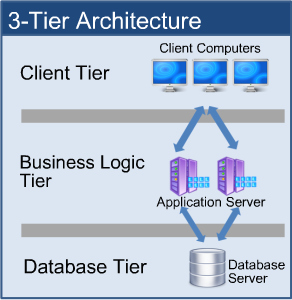
\includegraphics[scale=0.6]{img/3tier.jpg}
\label{Graphique technologie ajax}
\end{center}
 

\begin{list}{•}{}

  \item 
   La couche \textbf{présentation} des données : correspondant à la restitution et à l’affichage sur le clients, le dialogue avec l’utilisateur;
  
  \item
  Le \textbf{traitement} métier des données: correspondant à la mise en oeuvre de l'ensemble des règles de gestion et de la logique applicative;
  
  \item
  et enfin l’\textbf{accès aux données} persistantes : correspondant aux données qui sont destinées à être conservées sur la durée, voir de manière définitive   
  
\end{list}

Cette séparation a pour but de rendre indépendantes chacune des couches afin de simplifier la maintenance et les évolutions futures de l'application (par exemple, changement de système de base de données, portage d'un environnement graphique à un autre, ...).
Elle assure une sécurité plus importante car l'accès à la base de données n'est autorisé que par la couche Traitements.
Elle a également l'avantage d'optimiser le travail en équipe et de réduire les coûts de développement et de maintenance.


\section{Histoire de JavaScript}
\label{ch:histoire}

\subsection{Présentation}


Javascript (js pour les intimes) est un langage de script créé en 1995 par Brendan Eich pour le compte de Netscape Communications.

A cet époque Netscape Communications domine le marché du web. La firme fournie le navigateur web le plus populaire Netcape Navigator mais aussi des logiciels serveurs.

Netcape Communications lançait un partenariat avec Sun Microsystems pour exploiter leur nouveau langage ainsi que sa VM multi-plateforme, Java. Le but étant d’utiliser Java au sein du navigateur du coté serveur afin de fournir des UI riche portable ainsi qu’un moyen d’accéder à des applications via le web à travers un simple navigateur.

Cependant, Java est perçu par Sun et Netscape comme un langage peu adapté à une utilisation simple applicable à la page web car trop professionnel et contraignant. Java est à l’époque en concurrence avec Visual C++ de Microsoft. Il faut donc un langage plus simple à écrire, plus facile à utiliser pour les développeurs débutant et à prendre en main.

Netscape et Sun décide de créer un nouveau langage répondant à cette demande et en confie la création a Brendan Eich, gourou technique chez Netscape. La seule condition est que le langage doit être “dans le style java”  mais en moins puissant et clairement différenciés de java par les potentiels développeurs.

Comme l’a expliqué Brendan Eich dans une interview :


\begin{quotation}


JS devait « ressembler à Java », mais en moins avancé, [il devait] être le petit frère simplet de Java, son partenaire-otage. Et par-dessus le marché, je n’avais que dix jours pour pondre ça, ou on se retrouverait avec un truc pire que JS.

\end{quotation}

Javascript utilise la même syntaxe que Java (JS 1.0, mot-clés réservé et convention du JDK) mais il a du s’abstenir d’utiliser la syntaxe orientée-objet du langage, à une époque où la POO (Porgrammation Orientée Objet) était encore considérée comme un sujet réservé aux professionnels...

Brendan ne voulant pas pondre un langage diminué, il du trouver des ruses pour y glisser assez de puissance sans que celle-ci soit immédiatement visible au profane. Le langage devait rester simple et léger en apparence, tout en ayant assez de sophistication pour que des développeurs avancés soient à même d’en tirer des applications puissantes.

Même si Javascript et Java appartiennent à une famille syntaxique “de type C” (syntaxe des identifiants, accolades, opérateurs principaux, structures de contrôle...), ils ont des sémantiques extrêmement différentes. Javascript à une philosophie très fortement inspirée de langage objet ou fonctionnels “purs” au premier rang desquels Scheme et Self, mais aussi certains aspects de LISP et SmallTalk.

Java est un langage statique (chaque variable est typée), compilé et doté d’un typage fort, là ou JavaScript est dynamique, interprété avec un typage plus léger.

Java utilise un modèle d’héritage “classique”, mono-parent, basé sur l’héritage de classes. JavaScript est basé sur les prototypes et autorise plusieurs paradigmes de programmation notamment les stypes impératif, fonctionnel et orienté-objet.

Les deux langages sont donc extrêment différents, à un niveau philosophique, fondamental et pratique.

\subsection{Nom de code Mocha}

JavaScript est développé sous le nom de code Mocha. Son nom officiel étant LiveScript. Dans les deux premières versions beta de Netscapa Navigator 2.0, en septembre 1995, on trouve en effet LiveScript. A cet époque Miscrosoft n’avait pas encore collé une connotation négative à “Live”.

Cependant les marketeux ont voulu insister sur le rôle “collaboratif” de ca langage et tenter de récupérer un peu du prestige issu du marketing de Sun autour de Java. Du coup Brendan a du renommer LiveScript en JavaScript.

Peu de temps après (1996-1997), Netscape voulut faire bénéficier à JavaScript d’un processus formel de standardisation. ISO, IETF et le jeune W3C posaient chacun des problèmes distincts dans cet standardisation. L’ECMA (European Computer Manufacturers Association), un organisme de standardisation européen, en récupéra le bébé. Ainsi est sorti la première édition du standard ECMA-262 Ed. 1: ECMAScript est le nom de la norme officielle, JavaScript étant la plus connue des implémentations. ActionScript 3 est une autre implémentation bien connue de ECMAScript, avec des extensions.

Au fil du temps, il était clair cependant que Microsoft n’avait pas l’intention de coopérer ou de mettre en oeuvre correctement JS dans Internet Explorer même si Microsoft n’avait pas de proposition concurrente et avaient une partielle (et divergent à ce point) mise en oeuvre sur le coté serveur avec .NET.

Ainsi en 2003, le travail de JS2/original-ES4 à été mis en sommeil.

Le prochain évenement a eu lieu en 2005. Il s’agit en fait de deux évenements majeurs de l’histoire de JavaScript. Tout d’abord Brendan Eich et Mozilla rejoigne Ecma en tant que membre non-lucratif. Ont commencé alors les travaux sur E4X ECMA-357 en travaillant conjointement avec Macromedia

Ainsi, avec Macromedia (racheté par Adobe), le travail a redémarré sur ECMAScript 4, dans le but de normaliser ce qui était en AS4 et sa mise en oeuvre dans SpiderMonkey.

Hélas, en 2007, Doug Crokfort puis Yahoo ont uni leurs forces avec Microsoft pour s’opposer à ECMAScript 4, ce qui a conduit à la spécification ECMAScript 3.1 effort.

Pendant que les géant s’affrontait, la communautés de développeur open source c’est mise au travail pour révolutionner ce que l’on pouvait faire avec JavaScript. Cet effort collectif a été déclenchée en 2005, lorsque Jesse James Garrett a publié un livre blanc dans lequel il inventa le terme Ajax. Dans ce livre blanc, il décrit un ensemble de technologies, donc l’épine dorsale est JavaScript. La technologie est utilisé pour créer des applications web où les données peuvent être chargées en arrière-plan, en évitant la nécessité de recharger la page entière et aboutissant à des applications plus dynamiques. Suite à ce livre blanc, il en est résulté une période de renaissance de l’utilisation de JavaScript dirigé par les bibliothèques open source et les communautés qui se sont formées autour d’elles. Ainsi est né des bibliothèques comme Prototype, JQuery, Dojo, Motools et bien d’autres.

En juillet 2008, les parties conflictuelles se sont réunis à Oslo. Cela a conduit début 2009 à l’accord final de renommer ECMAScript 2.1 à ECMAScript 5 et à condire le langage vers l’avant avec la futur norme connu sous le nom de "Harmony".


La 3ème édition (ES3) consitue le socle de la version la plus utilisée/répandue du langage. La 4ème est morte-née, et la 5ème (ES5), désormais implémentés dans tous les navigateurs modernes, sert de socle aux applications web modernes ainsi qu’à JavaScript côté serveur (avec notament Node.js).

Tout cela nous amène à aujourd’hui, JavaScript entre dans un cycle complètement nouveau et passionnant dans son évolution, son innovation et sa normalisation, avec de nouveaux développement tels que Node.js, afin d’utiliser JavaScript coté serveur. L’arrivé de HTML5 dans le monde du web va également transformer l’évolution de JavaScript grâce au HTML5 APIs afin de controler les navigateurs coté-client, utiliser les web-sockets pour toujours plus de communications, obtenir des données sur des fonctionnalités tels que l'accéléromètre, la localisation GPS, et bien plus encore.

Actuellement JavaScript est disponible de base sur davantage de périphériques et de plates-formes que Java.

Même si l'explosion d’Android a fortement relancé le déploiement de Java qui s'enorgueillit de " plusieurs milliards de périphériques installés ”, Java n’est pas tellement déployé sur d’autres plates-formes mobiles, et n’est pas non plus automatiquement présent sur toutes les plates-formes desktop.

Allez trouver un seul desktop, laptop, smartphone, tablette ou liseuse qui n’ait pas une runtime JavaScript installé et qui s’en serve intensivement !

Dans certains cas, comme webOs, Firefox Mobile, JavaScript est au cœur-même de la plateforme, constituant sa clé de voûte.

iOS, Android, Windows Phone et Blackberry ont une tendance forte à utiliser des web apps reposant très lourdement sur JavaScript. Petit à petit, les technologies collectivement appelées “HTML5” remplacent ce pourquoi on avait encore recours aux applets ou, plus souvent, à Flash.

Ainsi commence la révolution JavaScript.

\section{EcmaScript}
\label{ch:ecmascript}

\subsection{Présentation}

ECMASCript est un langage de programmation de type script. Il est standardisé par Ecma International dans le cadre de la spécification ECMA-262. Il s’agit d’un standard, donc les spécifications sont mises en œuvre dans différents langages comme JavaScript ou ActionScript.

JavaScript évolue donc en fonction de l'avancement des standard de Ecma-International.

Comme vu précédemment JavaScript a vu le jour en décembre 1995 par Sun et Netscape.

En mars 1996, Netscape implémente le moteur JavaScript dans son navigateur web Netscape Navigator 2.0. Le succès de ce navigateur contribue à l’adoption rapide de JavaScript dans le développement web orienté client. Microsoft qui était à l’époque le seul concurrent a réagit en développant JScript, qu’il inclut ensuite dans Internet Explorer 3.0 en août 1996 pour la sortie de son navigateur.

Netscape soumet alors JavaScript à l’ECMA pour le faire standardiser. Les travaux débutent en novembre 1996, et se terminent en juin 1997 par l’adoption du nouveau standart ECMAScript. Les spécifications sont rédigées dans le document Standard ECMA-262.

ECMAScript existe à ce jour en 5 versions du standart ECMA-262.
\section{JSON}
\label{ch:json}

\subsection{Présentation}


JSON est un format d’échange de données qui est un sous ensemble de la notation objet littérale en JavaScript. Il a beaucoup gagné en popularité ces derniers temps comme une alternative légère au format XML, en particulier dans les applications AJAX.

Pourquoi ça?

En raison de la capacité de JavaScript pour l’analyse rapide de l’information à l’aide la fonction eval(). JSON ne nécessite pas cependant JavaScript, et il est possible de l’utiliser comme un format d’échange simple pour n’importe quel langage de script.

Voici un exemple de ce que JSON est:

\lstinputlisting[language=json]{code.json}

Voici à titre de comparaison sont équivalent en XML

\lstinputlisting[language=XML]{code.xml}



Certains développeurs pensent que JSON est une façon plus élégante d’écrire les données. D’autres apprécient sa simplicité. D’autres encore soutiennent qu’il est plus léger.

Peut importe, si JSON est si populaire c’est surtout grace à la technologie AJAX.


\chapter{Ajax}
\label{ch:ajax}

\section*{Introduction}

AJAX (Asynchronous JavaScript And XML) est une architecture informatique permettant de construire des sites web dynamiques interactifs et des applications Web en se servant de différentes technologies présenté précedment.

Ajax combine JavaScript, XML, CSS, le DOM et XMLHttpRequest afin d’améliorer la maniabilité et le confort d’utilisation des Applications Internet Riches (RIA).

Le terme Ajax a été introduit par Jesse James Garrett, le 18 février 2005, dans un article sur le site Web Adaptive Path. Ajax a créé une petite révolution dans les navigateurs.

En utilisant Ajax, le diaglogue entre le navigateur et le serveur se déroule la plupart du temps de la manière suivante:

 
Graphique techno ajax

Les échanges de données entre le client et le serveur peuvent utiliser d’autres formats notamment JSON.

Ajax à permi a JavaScript de gagner en popularité et de ne plus être le vilain petit canard des langages de programmation. Ainsi avec AJAX javaScript n’est plus une langage afichant des popup intempestives et vérifiant des formulaires.

Google a marqué les esprits avec Google Maps. Maps n’aurait jamais pu éxister sans Ajax. L’utilisation de JavaScript par Google a permis a JS de montrer son potentiel. Depuis JS s’est désinhibé, et de véritables logiciels sont apparus dans nos navigateurs.

Google est un très gros consomateurs de JS notament avec Drive ou Gmail.

JavaScript est donc passé du petit langage d’agrément pour pages web au langage de développement d’applications réseau supporté par tout les navigateurs quelques soit le système d’exploitation. Et le navigateur, pour un grand nombre d’utilisateurs, est la porte d’entrée de l’ordinateur et du réseau.

Avant AJAX: la page web est le support pour de petites applications Js, le plus souvent d’agrément et facultatives pour utiliser le contenu.

Avec AJAX: Js deviens le coeur du site. Il génère du contenu HTML dont il a la maitrise. Avec un autre langage coté serveur, Js coté client s’appuie sur le moteur graphique du navigateur pour générer l’interface de l’application, plus pratique que n’importe quel “toolkit”.

Cette mutation a pris du temps. Le navigateur est passé d’un logiciel pour consulter des pages web à un logiciel permettant d’exécuter d’autres logiciels (en somme comme un système d’exploitation).

Ajax est donc plébiscité parce qu’il donne naissance à des applications comme jamais nous avions vu par la fenere du navigateur. Avec AJAX une application comme Google Earth pourrait aussi bien exister de façon autonome.

Mais à cet époque, JavaScript à encore des inconvénient majeur empechant son adoption en masse.

JavaScript étant exécuter par le navigateur les performances à l’époque était extremement faible. Acuellement la bataille des navigateurs se au meilleurs support de HTML5/CSS3 mais aussi sur les performances des moteurs JS. L’arrivé de Google Chrome et des énormes besoins de Google en performance JavaScript ont poussé tout les acteurs du marché à améliorer les moteurs pour toujours plus de performances.

Le second problème de JS est l’éxécution du script par le moteur. Suivant le navigateur le code js doit être différent, chaque éditeur étant libre d’integrer JS comme il le souhaite. Ainsi un code js peut fonctionner correctement sur Firefox ou Chrome mais pas sur IE.

Le Javascript est aussi un langage qui nécessite des efforts importants et des développements en AJAX pur peuvent être extrêmement coûteux.

Afin de résoudre se problème de développement  John Resig à sortie un framework révolutionnant la façon d’écrire du code JavaScript. Ce framework: Jquery.


\section{JQuery}
\label{ch:jQuery}

\subsection{Introduction}

Au cours des dernières années, JavaScript a subi une transformation remarquable. Où une fois l'idée d'un langage jouet relégué au second plan, c'est aujourd'hui l'un des langage de programmation les plus importants dans la monde. 

Avec l'importance grandissante du développement basé sur Ajax, la montée des bibliothèques JavaScript augmentent et la stigmatisation entourant JavaScript à pratiquement disparu.

Il faut reconnaître que la bibliothèque la plus populaire et user-friendly, jQuery est en partie responsable de ce progrès.

jQuery est plus qu'un simple choix de débutant, il est en réalité utilisé par certaines des plus grandes organisations dans le monde, ajoutant de l'interactivité à des milliards de pages vues chaque mois. Google, Microsoft, Amazon, IBM, Twitter, NBC, Best Buy et Dell ne sont que quelques une des entreprises utilisant jQuery en production. Avec une très grande utilisation dans le monde, il n'est donc pas surprenant que jQuery évolue à une grande vitesse. 

jQuery continue de s'épanouir et les développeurs du monde entier contribuent aux fixes des bugs, des plugins et des travaux sur des projets connexes comme jQuery UI et QUnit. Ce regain d'activité assure que jQuery représente une option complète pour tout développeur cherchant à faire du développement JavaScript de catégorie mondiale.

Cela est vrai quelle que soit la philosophie ou la technique de développement utilisé: jQuery est utilisé peut importe le langage coté serveur tel que : Java/Spring, PHP, .NET, Ruby on Rails, Python/Django par exemple.

jQuery est une bibliothèque JavaScript qui porte sur l'interaction entre JavaScript (comprenant AJAX) et HTML, et a pour but de simplifier des commandes communes de JavaScript. Jquery se caractérise par un ensemble de fonctions qui permettent d’offrir une alternative à la programmation JavaScript de façon uniforme sur les navigateurs les plus courants et permet par exemple de manipuler aisément le DOM, de créer des animations etc… mais surtout de gagner du temps dans le développement des applications : « write less, do more ».

La librairie est sous licence GPL et MIT, et donc complètement réutilisable sur des travaux professionnels. De plus la librairie à l’avantage d’être compatible avec d’autre librairie JavaScript. 

\begin{itemize}
  \item[\textbullet]
  C'est une bibliothèque puissante. Le système jQuery réalise toutes sortes de tâches impressionnantes pour simplifier l'écriture de votre JavaScript.
  
  \item[\textbullet]
  Elle est légère. Il faut inclure une référence à votre bibliothèque dans chaque fichier qui l'utilise. La bibliothèque jQuery fait 26 ko (dans sa version compressée), une taille inférieure à certains fichiers image. Elle n'a donc aucun impact significatif sur la vitesse de chargement.
  
  \item[\textbullet]
  Elle prend en charge un mécanisme de sélection flexible. jQuery simplifie et développe le mécanisme document.getElementById, essentiel pour la manipulation du DOM.
  
    \item[\textbullet]
    Elle dispose d'un excellent support d'animation. Vous pouvez utiliser jQuery pour afficher et masquer, déplacer et glisser des éléments.
    
    \item[\textbullet]
    Elle rend les requêtes AJAX évidentes. Vous allez être surpris par la facilité d'utiliser AJAX avec jQuery.
      
    \item[\textbullet]
    Elle possède un mécanisme d'évènement amélioré. JavaScript dispose d'un support très limité pour les évènements. jQuery offre un outil très puissant pour ajouter un gestionnaire d'évènement à presque tous les éléments.
    
    \item[\textbullet]
    Elle fournit un support multiplateforme. La bibliothèque jQuery tente de gérer des questions de compatibilité de navigateur pour vous. Ainsi, vous n'avez pas à vous soucier d'éventuels problèmes de navigateurs.
    
    \item[\textbullet]
    Elle prend en charge les composants d'interface utilisateur. jQuery propose une bibliothèque d'interface utilisateur puissante qui compte des outils que HTML n'a pas, comme les contrôles glisser-déposer, les sliders et les calendriers.

    
    \item[\textbullet]
    Elle est évolutive. jQuery possède une bibliothèque d'extension qui accepte tous types de fonctionnalités optionnelles, y compris de nouveaux composants et outils tels que l'intégration de son, les galeries d'images, les menus, etc.
    
    \item[\textbullet]
    Elle introduit de nouvelles idées de programmation. jQuery est l'outil idéal pour découvrir des idées intéressantes comme la programmation fonctionnelle et les objets chaînables.
    
    \item[\textbullet]
    Elle est gratuite et open-source. jQuery est disponible en licence open-source, ce qui signifie que son utilisation est gratuite et que vous pouvez la consulter et la modifier si vous le souhaitez.
    
    \item[\textbullet]
    Elle est tout de même classique. Si vous décidez d'utiliser une autre bibliothèque AJAX, vous pourrez y exploiter les enseignements acquis dans jQuery.

\end{itemize}

\subsection{Document Object Model (DOM) }

Quand vous regardez un site web, vous voyez beaucoup d'éléments regroupés et assemblés pour former ce qui est en face de vous. Pour pouvoir accéder à ces éléments pour supprimer, ajouter et manipuler ces éléments, vous avez besoin d'un certaine formes d'interface, d'une représentation des éléments dans une page structuré et qui suit un ensemble de règle sur la manière de les modéliser. C'est ce qu'on appelle le DOM. Le DOM nous permet aussi de capturer dans le navigateur un événement comme lorsqu'un utilisateur clique sur un lien, soumet un formulaire, ou défiler la page.

Dans les premiers jours du web et des navigateurs, les normes en matières de mise en œuvre de JavaScript n'était pas efficace. Cela a conduit les navigateurs à intégré leur propre mise en œuvre de JavaScript créant des caractéristiques d'applications différentes causant des problèmes aux développeurs d'applications.
Ainsi pour développer une application JavaScript il  faut la coder pour chaque navigateur, ceux ci avait des implémentations différentes principalement entre Netscape et Internet Explorer.

Heureusement les choses ont progressé, les navigateurs optent actuellement pur les mêmes normes et les choses se sont stabilisés. Toutefois, le niveau auquel les navigateurs supportent le DOM peut encore pauser des problèmes aujourd'hui. En particulier avec les version d'Internet Explorer 6, 7 et 8 qui ne supporte pas le DOM au même niveau que les navigateurs les plus modernes. 

C'est une des raison pour lesquels jQuery est si précieux: tout ce quelle offre fonctionne aussi bien dans une version antérieur de Internet Explorer que la dernière version de Google Chrome ou Mozilla Firefox.

Afin d'avoir des bases solides pour la suite, je vais prendre la peine de présenter le façon dont le DOM est mise en œuvre.

Quand une page est chargée, le navigateur génère une représentation de ce qui est sur la page, et pour chaque élément il génère un ou plusieurs nœuds qui le représentent. Lorsque vous travaillez avec JavaScript, le DOM (suivant les implémentation différentes des navigateurs) peut provoquer des problèmes et conduire à passer beaucoup de temps sur des solutions de contournement, mais la beauté d'un framework comme jQuery permet de régler ce soucis.
Lorsqu'un navigateur forme une représentation de la page en cours avec le DOM, chaque élément est un nœud. Prenons l'exemple d'un paragraphe avec du texte un l'intérieur, tels que:

<p>Hello World</p>

Ce n'est pas un, mais deux nœuds. Il y'a un nœud de type texte qui contient "Hello World" et un nœud de type élément qui est la paragraphe. Le nœud de type texte est un enfant du nœud de type élément parce qu'il réside en son sein. Dans une page type, il existe beaucoup de nœuds imbriqués. Un div avec deux paragraphes composé de texte à l'intérieur s'articule comme ceci: 

div element node
-- paragraph element node
---- text node
-- paragraph element node
---- text node

Les deux paragraphes de cette instance sont frères parce qu'ils ont le même nœud parent. Les paragraphes sont enfants de la div, mais les nœuds de type texte ne sont pas des nœuds enfants parce qu'ils ne sont pas descendants directs de l'élément div.
Ils sont les nœuds enfants des nœuds de type paragraphe. Il existe trois principaux types de nœuds que vous devez savoir: élément, texte et attribut. 

\subsection{Les autres forces de jQuery }

Pour finir avec jQuery j'ajouterai quelques autres détails qui permettrons d'expliquer pourquoi jQuery à permit à JavaScript de prendre son envol.

\begin{itemize}

  \item[\textbullet]
  La documentation officielle est très fournie et de grande qualité ;
  
  \item[\textbullet]
  La communauté qui gravite autour de jQuery est en perpétuelle expansion et elle fournit un support de qualité ;
  
  \item[\textbullet]
  De nombreux acteurs de premier plan du Web (Microsoft, Google, Amazon, Twitter, Mozilla, etc.) utilisent jQuery ;
  
  \item[\textbullet]
  Une foultitude de plugins est disponible afin d'augmenter les possibilités de base de jQuery.  
  
\end{itemize}
\section{Restfull}
\label{ch:restfull}

\subsection{Présenation}

En 2000, Roy Fleding, l’un des principaux contributeurs aux protocoles HTTP et URI, a codifié l’architecture du Web dans sa thèse de doctorat intitulée “Architectural Styles and the Design of Network-Based Software Architectures.”

Dan cette thèse, il a introduit une architecture connu sous le nom "Representational State Transfer (REST)". Ce modèle, en termes abstraits, décrit les fondations du World Wide Web (WWW). Les technologies qui composent ces fondations comprennent le Hypertext Transfer Protocol (HTTP), Uniform Ressource Identifier (URI), les langages de balisages tels que HTML et XML et formats adaptés au Web comme JSON.

REST est un style d’architecture pour les applications en réseau. Il se compose de plusieurs contraintes pour assurer la visibilité, la fiabilité, l'évolutivité etc.

Cela rend REST attrayant pour construire des applications client/serveur distribué et décentralisé dans l'infrastructure du Web. Le déploiement de services Web sur cette infrastructure vous permet de profiter d’un large éventail d'infrastructures existantes qui comprennent les serveurs web, les clients, les bibliothèques, les serveurs proxy, les caches, les firewalls, etc.

HTTP est un protocole de niveau applications qui définit des opérations de transfert entre les clients et les serveurs. Dans ce protocole, les méthodes telles que GET, POST, PUT et DELETE sont des opérations génériques agissant sur les ressources. Ce protocole élimine le besoin d'inventer des opérations spécifiques à l’application tels que CreateOrder, getStatus, updateStatus, etc. Les bénéfices que vous pouvez tirer de l'infrastructure HTTP dépénd de comment vous utiliser le protocole HTTP. Cependant, un certain nombre de techniques, y compris SOAP et certains frameworks web Ajax utilisent HTTP comme protocole pour transporter des messages. 

\section{MVC}
\label{ch:mvc}

\subsection{Une structure}


Le secret pour faire de grandes applications JavaScript n’est pas d'en faire une volumineuse. Il s'agit plutôt de dissocier votre application dans une série de composants relativement indépendants. Les développeurs font bien souvent l’erreur de créer des applications avec beaucoup d’interdépendances, avec d’énormes fichiers JavaScript linéaires générant une flopée de balises HTML. Ces applications sont difficiles à maintenir et à étendre, et par conséquent devraient être évitées à tout prix.

Faire un peu attention à la structure de l'application lorsque vous commencez à la construire peut faire une grande différence sur le résultat final. Ignorez toutes les idées préconçues que vous avez sur JavaScript et traitez le comme un langage orienté object. Utilisez les classes, l’héritage, les objets et les modèles de la même façon que vous le feriez avec un autre langage, comme Python ou Ruby. L’architecture est essentielle du coté serveur alors pourquoi ne pas faire la même chose coté client? L’architecture retenue dans ce mémoire comme dans la plupart des frameworks présentés est l’architecture MVC, une architecture permettant de maintenir et étendre vos applications. Ce modèle s’applique particulièrement bien aux applications JavaScript.

\subsection{Qu’est ce que MVC ?}


MVC est un modèle de conception qui découpe une application en trois parties: les données (Modèle), la couche de présentation (Vue), et la couche d’interaction de l’utilisation (Contrôleur).

En d’autres termes, le flux dévénement est comme ceci:

\begin{enumerate}

  \item
  L’utilisateur interagit avec l’application

  \item
  Le gestionnaire d’évenements déclenche le Controleur

  \item
  Le Controleur demande les données du modèle, qui est envoyé à la Vue.

  \item
  La Vue présente les données à l’utilisateur.

\end{enumerate}

Ou en représentation graphique

\begin{center}
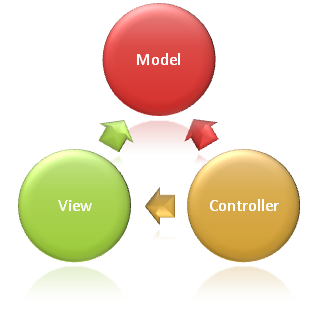
\includegraphics[scale=0.6]{img/mvc.png}
\label{L'architecture MVC}
\end{center}


Le modèle architectural MVC peut même être mis en oeuvre sans bibliothèques ni framework. La clé est de répartir les responsabilités des composants MVC en sections de code définis, en les gardant découpés. Cela permet de rendre indépendant le développement, les tests et la maintenances de chaque composants.


\section{Conclusion }
\label{ch:cintro}

\subsection{conclusion}

blabla




%client
\chapter{Client}
\label{ch:client}

\section{Introduction}

\section{Ember}
\label{ch:ember}

\subsection{Présentation}


Ember.js est un framework frontend MVC écrit en JavaScript qui s’éxécute dans le navigateur. Il est destiné aux développeurs qui cherchent à construire des applications web avec autant de puissance et de fonctionnalités que les applications natives concurrentes.

Ember.js a été créé à partir de concepts introduits par les applications natives telles que Cocoa. Ember.js vous aide à créer une grand expérience pour l’utilisateur. Il vous aidera à organiser toutes les interactions directes qu’un utilisateur peut effectuer sur votre site/applications.

Quand vous pensez que votre code JavaScript va devenir complexe, lorsque le code deviens long et compliqué, lorsque le refactoring du code s'annonce complexe alors Ember.js vous permet d'éviter de vous retrouver dans ces situations. Grave à sa structure MVC (Modèle-vue-controleur) il est facile de faire des modifications ou refactoring de code de n’importe quelle partie de votre code. Il vous permettra également d’adhérer aux principes du DRY (Don’t Repeat Yourself). Le modèle associé aux vues et aux contrôleurs exécute du CRUD (Create, Read, Update, Delete) pour l’informer d’un changement d’état. Il peut envoyer également une demande à la vue pour modifier la façon dont la vue représente le modèle actuel. La vue recevra alors des informations du modèle pour créer un rendu graphique.

Ember.js découpe les zones problématiques de votre interface vous permettant de vous concentrer sur une zone à la fois sans le souci d’affecter d’autres parties de votre application. Pour vous donner un exemple de certains domaines de Ember.js, jetez un oeil à la liste suivante:

\begin{itemize}

  \item[\textbullet]
  Navigation: le routeur d’Ember s’occupe de la navigation de l'application

  \item[\textbullet]
  Mise à jour automatique des modèles: Les vues d’Ember sont automatiquement mises à jour lorsqu’il y a une modification. Ce qui signifie qu’ember met à jour automatiquement les données sous-jacentes lorsqu'il y a un changement.

  \item[\textbullet]
  Manipulaton des données: Chaque objet créé sera un objet Ember, héritant ainsi de toutes les méthodes Ember.object.

  \item[\textbullet]
  Comportement asynchrone: Les liaisons et les propriété utilisées avec Ember aident à gérer l’asynchrone.

\end{itemize}

Ember.js est plus qu’une bibliothèque. Ember.js prévoit de construire une bonne partie du frontend autour de méthodes et d’une architecture carrées, créant ainsi une solide architecture une fois que vous avez terminé votre application. C’est la principale différence entre Ember et un framework comme Angular.js. Augular s’autorise à être incorporé dans une application existante alors que Ember doit être utilisé avec sa propre architecture et sa philosophie. Backbone.js serait un autre exemple de bibliothèque pouvant être facilement inséré dans des projets JavaScript existants.

Ember.js est un excellent framework pour la gestion complexe des interactions réalisées par les utilisateurs de votre application. Si vous pensez que Ember.js est un framework difficile à apprendre, c’est totalement faux. La seule difficulté pour les développeurs réside dans la compréhension des concepts que Ember.js cherche à mettre en oeuvre. Ember.js favorise convention plutôt que configuration.

\section{Backbone.js}
\label{ch:backbone}

\subsection{Introduction}

Backbone.js est un framework JavaScript permettant de structurer une application web non pas comme une suite d’instruction jQuery, mais comme un ensemble de vues autonomes les unes des autres.

Backbone est un bon choix pour les applications dites ‘single page application”.

Single page application ( Application Web Monopage) c’est à dire pour simplifier, une page principale avec un nombre important d'interactions utilisateur. Plutôt que d’’avoir une navigation par page (le serveur envoie une page à chaque URL), la navigation, l’envoi de formulaire et toutes les actions classiques se gèrent en javascript.

Avant, lorsque l'on souhaitait faire ce genre de choses, on écrivait son propre JavaScript, sans aucune convention, à grand coup d’AJAX et de script Jquery. On se retrouvais vite avec un code complexe à maintenir et à tester.

Backbone.js permet de cadrer cela en définissant modèle, vue et collections afin de structurer notre code. On va pouvoir définir des événements sur des changements de valeurs de nos modèles et ainsi rafraîchir automatiquement nos vues.

Backbone.js possède son routeur. On peut faire correspondre des actions à des URL.

Il se veut non-contraignant par rapport à ses rivaux, ce qui lui coûte d’être présenté souvent comme moins complet. Son point fort est d’être facilement utilisable avec d’autres libraires ou frameworks.

Par contre Backbone.js est uniquement une couche client. Il ne gère pas la persistance des données sur un serveur. Heureusement cela se gère très bien en utilisant l’architecture REST. Il suffit d’indiquer à nos modèles une URL et d’utiliser une API JSON Restful pour être capable de réaliser du CRUD très facilement. 


\subsection{Dépendances}


Backbone.js est basé sur la blirairie Undercore.js. Cette dernière propose des fonctionnalités de manipulation d’objets, de collections et de tableaux assez poussées. Comme toute librairie populaire, elle se veut cross-browser et par héritage, Backbone.js l’est aussi.

Pour tout ce qui est manipulation DOM, plutôt que réinventer la roue, l’équipe en charge de Backbone.JS a décidé de sous traiter cette tâche à jQuery. Il est possible de remplacer jQuery, par exemple avec Zepto, du moment qu’elle respecte l’api jQuery-compatible.

\subsection{Composants}


Backbone.js fournit des composants logiciels pouvant être utilisés librement, que ce soit avec les autres composants Backbone.js ou avec une autre librairie. Les trois plus importants sont le Model, La Vue et la Collection.

Les composants Router et Sync fournissent des fonctionnalités très intéressantes.


\subsection{Les données}


La classe Backbone.Model est utilisé pour gérer du contenu sous la forme d’un objet JavaScript, en l’encapsulant et en proposant des méthodes accesseurs.

La classe Backbone.Collection permet de manipuler des collections de Model. On retrouve les méthodes habituelles: push, pop, shift, unshift, add, remove, get, sort ou encore length. On retrouve également les fonctions provenant de Underscore.js

Ces deux classes permettent de manipuler des données. Mais Sync permet de le faire plus simplement.

Sync est le composant permettant de synchroniser les objets à travers une API du type RESTful JSON. Pour cela, il suffit de lier les objets Model et Collection à une ressource grâce à l’attribut url.

\subsection{La vue}

Toutes les manipulations DOM se font à travers le plugin jQuery qui est de loin, le mieux armé pour ces opérations.

Chaque objet Backbone.View est lié à un nœud DOM (el) et pourra le générer à nouveau, à n’importe quel moment. Le but est alors de découper le document en une multitude de vues que l’on pourra régénérer à souhait et individuellement. 

\subsection{Asynchronous Module Definition API}

Il est possible d’utiliser Backbone.JS avec un AMD Loader comme RequireJS ou Curl. Ni Backbone.JS, ni Underscore ne supportent officiellement AMD. Toutefois, il est possible d’utiliser un fork implémentant de cette API.
On trouve sur Github des projets templates (boilerplate) qui facilitent la mise en place d’un environnement couplant RequireJS et Backbone. 

\subsection{Plugins}

Backbone.JS se veut léger : il ne fournit que des composants essentiels. Un des gros manquements de Backbone.JS par rapport à ses concurrents est l’absence de la fonctionnalité de DataBinding. Mais qu’à cela ne tienne, de nombreux plugins sont présents en libre accès sur GitHub, pour implémenter des fonctionnalités. 

\section{AngularJS}
\label{ch:angularjs}

\subsection{Introduction}

AngularJs est un framework structurel pour les applications web dynamiques. Il est écrit en JavaScript et est sous Licence MIT.

C’est un framework open-source au même titre que MooTools, Prototype, Dojo ou Jquery.

AngularJs est développé par Google et sa communauté.

AngularJS permet d’utiliser le HTML comme langage de template et vous permet d’étendre la syntaxe du HTML pour exprimer les composants de votre application de façon claire et succincte.

Il a pour but de simplifier l’écriture du JavaScript en simplifiant la syntaxe et de combler les faiblesses de ce langage en lui ajoutant de nouvelles fonctionnalités. Le but d’AngularJs est de faciliter la réalisation d’applications web monopages.

AngularJs peut être utilisé avec ou sans jQuery pour la manipulation du DOM.

Le framework adapte et étend le HTML traditionnel pour servir le contenu dynamique de façon améliorée grâce à un data-binding bidirectionnel qui permet la synchronisation automatique des modèles et des vues. En conséquence AngularJS minore l’importance des manipulations DOM et améliore la testabilité du code.

AngularJs essaie d’être une solution complète pour créer une application web. Il est livré avec tout ce dont vous avez besoin pour construire une application CRUD de façon cohérente: liaison des données, directives de bases pour les templates, la validation du formulaire, le routage, le deep-linking, la réutilisation de composants et l’injection des dépendances. AngularJs permet l’écriture de tests unitaire, cas de test, mocks etc.



\subsection{Objectifs de conception du framework}
\begin{itemize}

	\item[\textbullet]
    Découper les manipulations du DOM de la logique métier. Cela améliore la testabilité du code.
    
	\item[\textbullet]
    Guider les développeurs pendant toute la durée de la construction d'une application: de la conception de l'interface utilisateur, en passant par l'écriture de la logique métier, jusqu'au test de l'application.

	\item[\textbullet]
    Considérer le test d'une application aussi important que l'écriture de l'application elle-même. La difficulté de la phase de test est considérablement impactée par la façon dont le code est structuré.

	\item[\textbullet]
    Découper les côtés client et serveur d'une application. Cela permet au développement logiciel des côtés client et serveur de progresser en parallèle, et permet la réutilisation du code de chaque côtés.

	\item[\textbullet]
    Rendre les tâches faciles évidentes et les tâches difficiles possibles.

\end{itemize}

AngularJS est un framework MVC et encourage le couplage faible entre la présentation, les données, et les composants métiers. En utilisant l’injection de dépendances, AngularJS apporte aux applications web coté client les services traditionnellement apportés coté serveur, comme les contrôleurs de vues. En conséquence, une bonne partie du fardeau supporté par le back-end est supprimé, ce qui conduit à des applications web beaucoup plus légères et maintenables.


\section{CanJS}
\label{ch:canjs}

\subsection{Présentation}

Le framework CanJS est issu du framework Javascript MVC. Il s'agit en fait de l'extraction du noyau et il est décomposé en modules pour correspondre exactement aux besoins de l’application sans embarquer d'importants volumes de fonctionnalités inutiles. La nouvelle version de Javascript MVC se basera sur CanJS pour assurer l’inter-compatibilité des deux frameworks.

Le grand intérêt de CanJS est de fournir des objets « Model » pour stocker nos données, y associer des fonctions de mise à jour coté serveur personnalisables et des événements auxquels attacher des actions. Mieux, il gère automatiquement, grâce à son système de templates, la mise à jour de toutes les vues associées à un modèle lorsque ce dernier est modifié.

CanJS est composé de:
\begin{itemize}

    \item[\textbullet]
can.Construct - hérite des fonctions du constructeur

\item[\textbullet]
    can.Observe - clé valeur contraignante

\item[\textbullet]
    can.Model - permet de connecter une interface JSON-REST

\item[\textbullet]
    can.View - chargement du modèle, mise en cache

\item[\textbullet]
    can.EJS - modèles contraignant direct

\item[\textbullet]
    can.Control - liaisons d’évènements déclaratif
    
\item[\textbullet]
    can.Route - support du bouton précédent et des onglets
    
\end{itemize}

Il prend également en charge un riche ensemble d’extensions et de plugins.

\subsection{Caractéristiques vs Poids}


En plus de jQuery, CanJS fait 8.5kb. A titre d’exemple voici quelques autres bibliothèques MVC (compressé avec gzip):

\begin{itemize}

	\item[\textbullet]
	8.97kb pour Backbone (avec Underscore.js)

	\item[\textbullet]
    24kb pour AngularJS

	\item[\textbullet] 
    13kb pour Knockout

	\item[\textbullet] 
    37kb pour Ember
    
    \item[\textbullet] 
    15kb pour Batman

\end{itemize}

Pour être juste, le poids est trompeur, car chaque bibliothèque possède un ensemble différent de fonctionnalités. Cependant, CanJS fournit tout ce dont vous avec besoin pour créer une application coté client riche, avec la bibliothèque la plus légère parmi celles que nous avons comparées.
Par comparaison Backbone.js est livré le micro template Underscore.js, mais celui-ci ne se compare pas à la puissance de EJS. La plupart des applications réseau de base comprennent également un moteur de templates qui ajoute du poids à la bibliothèque.

\subsection{Facilité d’utilisation}

CanJS bénéficie d’une courbe d’apprentissage plus facile que n’importe quelle autre biblothèque. Il bénéficie d’une bonne documentation, et il permet de se faire la main avec la page de présentation, puis de plonger plus profondément en lisant chaque méthodes et classes dans la page de documentation. CanJS permet de voir comment les applications sont construites en parcourant les exemples, en lisant les annotations et en regardant les jeux de tests. Un blog permet d’en savoir toujours plus sur CanJS, et il est possible de poser des questions sur le forum, Twitter ou d’obtenir un support premium, de formations ou de conseil.

\subsection{Prévention des fuites mémoire}

CanJS empêche les fuites de mémoire qu’un développeur ne connait problablement pas et a dans son application. Les applications JavaScript ont communément des fuites mémoire de deux sources: les gestionnaires d’évenements et les objets inutilisés.
Autant dire qu’il s’agit d’un problème critique pour les client MVC. CanJS gère ces fuites automatiquement ce qui rend presque impossible une fuite mémoire dans l’application.

\subsection{Performance}

CanJS est optimisé pour la performance dans des domaines clés.
Par exemple la liaison en temps réel est optimisée pour les performances en modifiant directement et exactement ce qui doit être mis à jour, plutôt que le modèle en entier.

Voici un schéma mesurant les performance de CanJS en fonction d’autres frameworks.


\begin{center}
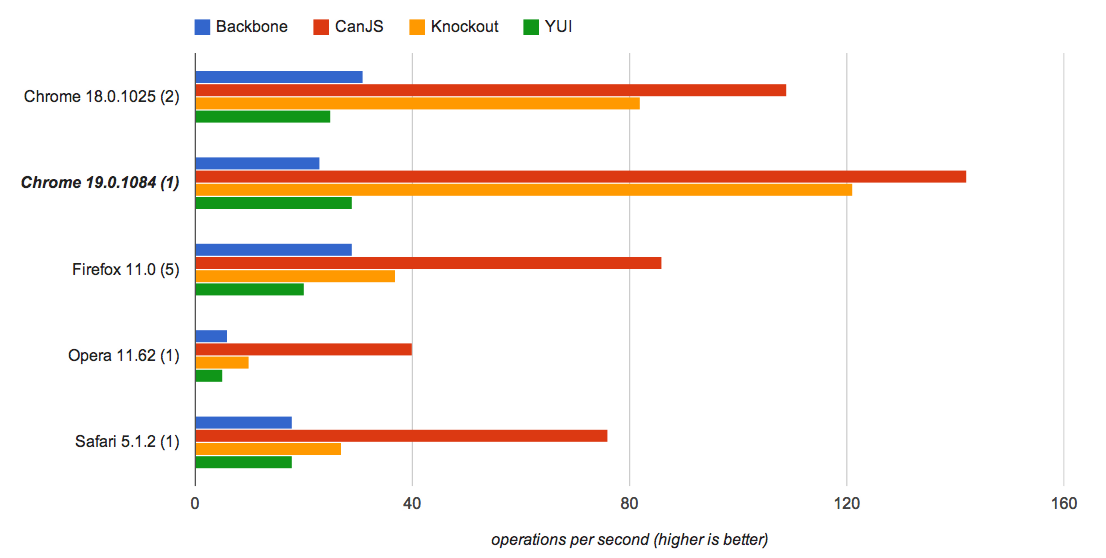
\includegraphics[scale=0.4]{img/performance_livebind.png}
\label{Graphique performance CanJS}
\end{center}

\subsection{Support de librairie}

CanJS permet d'intègrer cinq des bibliothèques les plus couramment utilisées pour l’accès au DOM:

\begin{center}

\includegraphics[scale=0.5]{img/CanJSlibraries.png}
\label{Graphique bibliothèque CanJS}
\end{center}

Cela donne la possibilité de choisir la bibliothèque préférée ou passer même facilement par une autre bibliothèque sans avoir a réécrire la couche MVC de votre application.

Il y a une intégration profonde avec chaque bibliothèque afin de permettre une utilisation complète et ce peu importe la librairie choisie.
\section{Conclusion}
\label{ch:conclusion client}

\subsection{Conclusion}



%serveur
\chapter{Serveur}

\section{Introduction}
\label{ch:introServeur}



Il y a encore quelques années, l’idée de faire du développement en Javascript faisait hérisser les cheveux de la plupart des programmeurs. Les développeurs se seraient volontiers passé de JavaScript si une alternative viable existait. Grâce à l'évolution technologique, l'explosion et la démocratisation des RIA (Rich Internet Applications) et la révolution du marché des navigateurs avec Chrome et Firefox, le JavaScript est devenu un langage de première classe dans le paysage web.

A la base JavaScript est également un langage prévue pour tourner coté serveur. Alors pourquoi ne pas développer un serveur d’application en JavaScript ?

Car malgré ses défauts, JavaScript est un langage possédant une expressivité impressionnante, \textbf{orienté objet}, doté de principes hérités des langages fonctionnels (Lisp, etc.) comme la \textbf{closure} ou les \textbf{lambda-functions}, et intégrant le paradigme de \textbf{programmation événementielle}... Bien loin, d’un langage pour faire de l’accès DOM. 

Ce chapitre a pour but de présenter le développement coté serveur avec  Node.js, une technologie basée sur V8, le moteur JavaScript de Google Chrome, dont elle étend les capacités en ajoutant de nombreuses fonctionnalités d'I/O (Entrées/Sorties).

Node est tellement important et performant qu’un mémoire/livre entier n’arriverait pas à couvrir son ensemble.

Ce chapitre va présenter \textbf{Node.js}, son gestionnaire de paquet \textbf{NPM} ainsi que deux framework assez prometteur \textbf{Express} et \textbf{Meteor} permettant de simplifier le développement d’application serveur avec Node.

\section{Node.js}
\label{ch:nodejs}

\subsection{Présentation}

Node.js est une plateforme open source pour le développement d’application coté serveur.

Il a été créé par Ryan Dahi en février 2009 et est depuis devenu très populaire. L’esprit de Node est similaire à Twisted pour Python et Eventmachine pour Ruby.

Il se compose délibérément d’une bibliothèque de base minimaliste accompagné d’un écosystème riche. Il fonctionne au dessus du moteur V8.  V8 est un moteur JavaScript très rapide développé par les ingénieurs de chez Google.

Le moteur JavaScript V8 de Google utilisé dans Chrome fait partie des moteurs JavaScript les plus puissants du marché.

JavaScript est populaire coté client, mais depuis peu il est un langage plébiscité pour le développement coté serveur.

Node permet de développer très simplement des applications scalables. : l'idée est d'utiliser des IO non bloquantes pour gérer toutes les requêtes entrantes, sortantes ainsi que tout le processus lié à la requête.




La page d’acceuil de Node.js le décrit ainsi:

“Node.js est une plateforme construire sur le moteur JavaScript de Chrome pour construire facilement des applications réseau rapides et évolutives. Node.js utilise une gestion d'événement basé sur des I/O non bloquantes, qui le rend léger et efficace, idéal pour les applications de données intensives en temps réels qui s’éxécutent à travers des dispositifs distribués. http://nodejs.org

Cela peut sembler énigmatique aux nouveaux arrivants, mais il résume succinctement certaines principales forces de Node.js et mérite d'être explorée plus en détail. Les gens sont souvent surpris quand ils entendent que JavaScript est un vrai langage de programmation complet et entier. Pour la communauté des développeurs, JavaScript n’est pas un vrai langage comme C, C++ ou Java.

Depuis ses humbles débuts, JavaScript a évolué et est désormais pris en charge dans tout les principaux navigateurs, y compris ceux sur les appareils mobiles. non seulement il est un langage populaire, mais les outils et frameworks actuellement disponibles sont nombreux et efficace, il est reconnu comme un langage puissant. JavaScript en tant que plateforme de développement coté serveur prend en charge l’intégration continue, le déploiement continu, les connexions aux bases de données relations, les architectures orientés services  et à peu prêt toutes les techniques disponibles.

En conjonction avec le moteur JavaScript V8 de Google, il est maintenant extrêmement rapide. En fait il est plusieurs fois plus rapide que les autres langages de script comme Ruby et Python. Contre Python 3, le moteur JavaScript V8 est environ 13 fois plus rapide avec un code similaire. Node.js est plus rapide d’environ 8 fois que Ruby 1.9. Ce sont des points de repère incroyable pour un langage dynamique, et est dû en grande partie à des optimisations du moteur v8.

La description officielle des discussions sur le modèle événementiel à I/O on bloquant est le suivant: Traditionnellement, la programmation se fait de manière synchrone: une ligne de commande est exécuté, le système attend le résultat, le résultat est traité, puis l’exécution reprend.

Parfois, attendre le résultat peut reprendre après un certain temps, par exemple, la lecture d’une base de données ou d’écriture sur un réseau.

Dans des langages tels que Java et C\#, une solution consiste à lancer un nouveau thread. Un thread peut être considéré comme un processus léger qui exécute des taches. Programmer en utilisant des thread peut être difficile parce que plusieurs thread peuvent essayer d’accéder simultanément à la même ressource. Sans disséquer les subtilités de la programmation multi-threading, vous pouvez imaginer que ce serait désastreux pour un thread à incrémenter alors qu’un autre thread décrémente le compteur en même temps.



\subsection{Architecture de Node.js}

\begin{center}
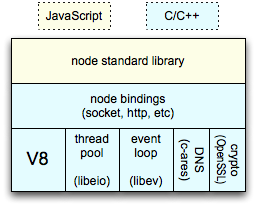
\includegraphics[scale=1]{img/nodejsarch.png}
\label{Graphique technologie node.js}
\end{center}

Node.js est en grande partie écrit en C/C++.
Mais il possède un framework complet en JavaScript pour développer nos applications. C'est ce qui le rend particulièrement intéressant.

\subsection{Boucle d’évènement}

Node est écrit en C++ et utilisant la bibliothèque libev de Marc Lehman, la boucle d’évenement utilise epoll ou kqueue comme mécanisme d’évenement évolutifs.

\subsection{I/O non bloquant}

Node évite de perdre en temps de calcul CPU habituellement rencontré par l’attente d’une réponse d’entrée ou de sortie (base de données, système de fichier, service web, …) grâce à l’asynchrone complet fourni par la bibliothèque libeiode Marc Lehmann 

Ces caractéristiques  permettent à Node de gérer une grande quantité de trafic en manipulant le plus rapidement une demande afin de libérer le thread pour la demande suivante. Node.js est un serveur capable de répondre au problème C10K.

Node possède un support intégré de la plupart des protocoles importants comme TCP, DNS et HTTP (celui qui nous interesse ici). L’objectif de la conception d’une application Node est que toute fonction effectue une E / S doit utiliser un callback. C’est pourquoi il n’existe pas de méthode de blocage prévu dans l’API de Node.

\subsection{Asynchrone}

Prenons l'exemple du serveur Apache. Chaque requête HTTP entrante se voit allouer un thread. Celui-ci est utilisé pendant toute la durée du traitement de la requête : lecture/écriture en base de données, lecture/écriture dans des fichiers de logs ou autres, exécution de code... Ainsi, si votre code côté serveur fait un accès à la base de données, celui-ci est en attente de la réponse. De plus, durant toute la durée de la requête, le client sera bloqué, en attente de la réponse du serveur.

Node et plus globalement les serveurs dits non bloquants (comme Netty ou Deft pour ceux qui tournent sur JVM) adoptent une autre approche. Node n'utilise qu'un seul thread pour gérer les requêtes entrantes. De plus, Node ne propose pas, dans ses API, de fonctions bloquantes. Ainsi, tout notre code est asynchrone. L'avantage immédiat à cela est la simplification à l'extrême de la gestion de la concurrence dans nos applications qui n'est ici plus gérée par le développeur mais directement par l'OS.

Concrètement, toutes les fonctions fournies par Node prennent en paramètre un callback. Une fois que la fonction termine son traitement, le callback sera appelé avec le résultat en paramètre et une éventuelle erreur. Ainsi, pendant toute la durée du traitement, le thread est relâché et peut être donné à une autre requête pour effectuer un autre traitement. Nous sommes donc face à un système évènementiel. Et Javascript est un très bon choix de langage du fait que l'on peut programmer de manière fonctionnelle avec celui-ci. Les callbacks dans tous les sens sont bien connu avec l’utilisation de librairies comme jQuery qui nous habituent depuis déjà quelques temps à ce type de développement.

\subsection{Performance}

Node.js est rapide. L'une des critiques les plus fréquentes à propos des langages interprétés comme PHP, Python et Ruby est la performance. Jason Hoffman, directeur de la technologie de Joyent, a discuté de la façon dont Node.js est ultra performant et peut être ralenti à cause des systèmes d'exploitation. Un seul core avec moins de 1 Go de RAM est capable de gérer 10 Go de trafic et un million de terminaux connectés. La combinaison de 24 d'entre eux sur une seule machine produit un niveau global de débit qui dépasse les capacité des systèmes d'exploitation et Piles TCP / IP. En d'autres termes, avec une application bien conçue, ce n'est pas Node.js le goulot d'étranglement c'est votre système d'exploitation.

\subsection{Communauté}

Malgré sa jeunesse, la communauté Node grandis de plus en plus rapidement et le dépot de Node est le 3ème dépot le plus suivi sur Github.

\subsection{Forces}

\begin{list}{•}{}
  \item
  Bien que Node.js date seulement de 2009 :
    \begin{list}{•}{}
      \item
      il a déjà un bon système de package : Node Package Manager que la grande majorité de la communauté semble utiliser
      \item
          il a déjà une très forte communauté, de très nombreuses librairies, exemple : plein de librairie classées, déjà plus de 9000 packages sur npm
      \item
      de plus en plus de sociétés semblent l'utiliser comme Linkendin par exemple.
    \end{list}
    
    
  \item 
  tous les développeurs web (front-end) connaissent le langage, il est très populaire. Par conséquent, pour passer à Node.js il n'y a pas le frein d'apprendre un nouveau langage comme ça serait le cas avec l'utilisation d'un framework web basé sur Ruby ou Python. Je pense que dans les mois qui viennent, de nombreux développeurs PHP vont passer à Node.js… surtout ceux qui regardaient ailleurs mais qui ne souhaitent pas apprendre un nouveau langage.

  \item
      la possibilité de partager du code (librairies communes…) entre la partie client et serveur peut être intéressant. La question se pose de plus en plus étant donnée qu'on est de plus en plus amené à effectuer beaucoup de traitement coté client (exemple avec Backbone.js).
      
  \item
  Ces derniers jours, la visualisation de screencast sur le framework JavaScript Meteor m'a profondément intéressé.
  
  \item
  Autre exemple, il est possible d'utiliser la même API Canvas coté client et coté serveur (avec node-canvas).
  
  \item
  Node.js semble être très rapide, ça tient très bien la monté en charge.
  
  \item
  La vitesse de l'interpréteur Javascript est en constante progression V8.

\end{list}

\subsection{Retour d'expérience Linkedin}
\section{NPM}
\label{ch:npm}

\subsection{Présentation}

Node Package Manager (NPM) est un gestionnaire de modules pour Node. C'est en quelque sorte un équivalent pour Node de aptitude ou apt-get (les gestionnaires de paquets sous Debian et Ubuntu) avec une interface très similaire. 

NPM permet d’ajouter de nombreuses fonctionnalités à Node (exemple : gestion des sockets avec socket.io, utilisation d’un framework avec Express JS, utilisation de template avec Jade…) en utilisant une commande npm qui s’occupera de télécharger et installer les modules demandés.

Par exemple pour télécharger la dernière version d'Express, il suffit d'exécuter la commande \textit{npm install express} et de laisser l'utilitaire faire son travail. Si quelques mois plus tard, le désire d’obtenir la dernière version d'express se fait sentir, on exécutera simplement \textit{npm update express}.

Cet outil  permet également d’installer directement un exécutable du module grâce a l’option \textit{-g} (très pratique pour Coffee-Script par exemple).

Actuellement le nombre de modules Node.js disponible est supérieur à 30 000 modules.

NPM, ainsi que des informations concernant son installation et son utilisation sont disponibles sur github, comme la grande majorité de l'écosystème node.





\section{Socket.IO}
\label{ch:socketio}

\subsection{Présentation}

Socket.IO est un module Node puissant qui apporte la possibilité de gérer simplement les connexions entre le serveur et le client.

D’après les dire du créateur de Socket.IO, “l’objectif est de fournir pour les applications basées sur les navigateurs, un mécanisme de communication bidirectionnelle entre des serveurs et/ou des clients". 
\textbf{Websocket} est un protocole bidirectionnel moderne qui permet une communication interactive  entre le navigateur et le serveur. Son principal inconvénient est que la mise en œuvre est généralement disponible uniquement sur les navigateurs les plus récents.
Cependant en utilisant Socket.IO, ce détail de bas niveau n’est pas un problème pour le développeur qui est soulagé par Socket.IO de la nécessité d’écrire du code spéficifique en fonction du navigateur.

Le côté client utilisera automatiquement et de manière transparente le meilleur type de communication (basé sur les fonctionnalités du navigateur) pour se connecter à un serveur Node.


Prenons un exemple
Si l’architecture de l’application utilise un client Google Chrome, le navigateur est capable d’utiliser le  protocole WebSocket et par conséquent Node choisira ce type de connexion.

Mais que se passerait il si l’on décide de créer une connexion avec le navigateur de Mozilla Firefox où le support des WebSocket est désactiver? Socket.IO choisira d’utiliser alors le mode de connexion en “long pooling”  automatiquement et ce sans besoin de changer quoi que ce soit dans le code du client et du serveur.

\section{Meteor.js}
\label{ch:meteor}

\subsection{Présentation}

Bien que peu connu, Meteor est un environnement très simple qui permet de développer des applications modernes en quelques heures, alors que ça prendrait plusieurs semaines avec de très bons outils. 
En effet, les applications développées avec Meteor s’éxécutent directement dans le navigateur plutôt que sur un serveur web et récupèrent toutes les données nécessaires dans le cloud.
Meteor est un framework open source qui mise beaucoup sur le JavaScript. Avec quelques lignes de JavaScript et quelques commandes, il est possible de développer une application Web relativement simple qui s’actualise en temps réel.
Un tel modèle est déjà utilisé par des grandes entreprises telles que Twitter, Facebook et Google mais était jusqu’alors hors de portée pour un développeur moyen. Avec cette levée de fonds conséquente (11,2 millions de dollars), le projet espère devenir plus accessible aussi bien aux débutants qu’aux experts et devenir, pourquoi pas, un standard.

En attendant, Meteor est toujours en cours de développement mais se développe rapidement et des changements majeurs sont au rendez-vous dans l’API à chaque nouvelle version. Ce n’est pas encore une version stable, il faudra pour cela patienter sans doute plusieurs mois. Mais je trouve interessant de le présenter dans ce mémoire.

\subsection{Principes}

Meteor permet de développer avec le même langage (en Javascript ou dans un langage compilant vers Javascript comme CoffeeScript ou Dart) et avec la même API sur le client et sur le serveur. Ce choix d’architecture permet de déplacer facilement un traitement du serveur vers le client (et réciproquement) voire de le dupliquer par exemple dans le cas de la validation d'un formulaire.
Dans cette logique, Meteor inclut un système de gestion de base de données côté client, fonctionnalité originale du framework. Il est ainsi possible d'effectuer des requêtes même en étant déconnecté du serveur. Cela permet notamment à Meteor d'inclure par défaut, des mécanismes de compensation de latence. Par exemple l'envoi d'un message dans un chat sera instantanément ajouté au fil des messages au clic sur le bouton "Envoyer", tandis que la vérification du message se fera en arrière plan côté serveur. Ce mécanisme permet l'utilisation de la programmation réactive coté client.

\subsection{Live HTML}

Si des modifications sont apportez au code HTML, CSS, JavaScript, ou à des données sur le serveur, chaque client montre les changements automatiquement sans actualisation du navigateur. Par exemple, si le développeur change la couleur de fond d'une page en jaune alors chaque navigateur affichera la nouvelle couleur de fond jaune sans aucun rafraîchissement. Ou, si un utilisateur ajoute un nouveau film à une collection de films, alors tous les navigateurs afficheront le nouveau film automatiquement.
Avec Live HTML, les utilisateurs n'ont plus besoin d'un bouton d'actualisation. Les modifications apportées à une application se produisent partout automatiquement sans aucun effort. Le framework Meteor gère tous les détails nativement afin de garder tous les clients  synchroniser avec le serveur simplement et sans aucun développement spécifique.

\subsection{Compensation de la latence}
Lorsque que quelqu'un réalise une modification des données sur le client, ces modifications apparaissent comme si elles se sont produites sur le serveur, sans aucun retard. Par exemple, si un utilisateur cré un nouveau film, le film apparaît instantanément. Cependant, ce n'est qu'une illusion. Dans le fond, les mises à jour de meteor actualise la base de données avec le nouveau film. Si, pour une raison quelconque, le film ne peut pas être ajouté à la base de données, Meteor enlève le film dans le client automatiquement.
La compensation de la latence est extrêmement importante pour la création d'une application Web sensible. Lorsque l'on veut que l'utilisateur soit en mesure d'apporter des modifications instantanées dans le navigateur, le framework va gérer les détails de la mise à jour de la base de données sans ralentir l'utilisateur.

\subsection{Temps réel}


Plutot que d’envoyer du html a votre client, Meteor propose d’envoyer seulement les données et de laisser le client décider de la façon dont elles doivent être affichées. La où Meteor est intéressant, c’est pour sa gestion native du temps réel. L’objet affiché dans votre navigateur a été modifié par un autre utilisateur ? Pas de problème, Meteor va informer tout les clients de cette modification, et affiche la modification en conséquence. Meteor a fait le choix d’utiliser SockJS. A la différence de socket.io, SockJS ne passe pas par les websockets, mais par les requêtes xhr par soucis de compatibilité avec tous les navigateurs. Tout se passe par un système de push/subscribe que l’on retrouve de plus en plus. L’intéret du push/subscribe est que les clients s’abonnent à des événement qui les intéressent et réagissent en conséquences.

\subsection{Rafraichissement automatique}

Lorsqu'un développeur est en train de développer, la sauvegarder d’un fichier sur son ordinateur va automatiquement rafraichir le navigateur avec ses modifications. Ce principe de modification à chaud est aussi disponible en production : Meteor annonce qu’une nouvelle version d'une application peut être déployée de façon transparente à ses utilisateurs.



%base de données
\chapter{Base de données}

\section{Introduction}
Une base de données est un conteneur permettant de stocker l'intégralité des informations d'une application sur un serveur.
Il existe plusieurs sortes de base de données, mais j'ai décidé de n'en présenter que trois. Ce sont celles utilisées en majorité dans les entreprises.
Il s'agit des bases de données relationnelles (MySQL,PostgreSQL,Oracle, SQLserveur...), des bases de données NoSQL (MongoDB...), et enfin récement de Webstorage.


\section{SGBDR}
Le monde du Système de Gestion de Base de Données Relationnelles est actuellement boulversé par l'arrivée du NoSQL et de nouveaux serveurs comme Node.js.
Mais la plupart des éditeurs de base de données ont compris la nécessité de s'adapter et proposent actuellement une réponse au NoSQL et à Node.js.


\begin{center}
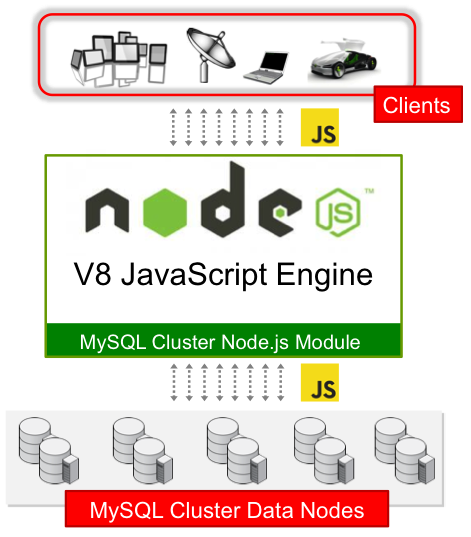
\includegraphics[scale=0.6]{img/mysql_cluster_73_nodejs_figure1.png} 
\label{Graphique technologie mysql cluster}
\end{center}

Afin d'éviter la fuite des développeurs vers des serveurs NoSQL, Oracle par exemple a développer un connecteur NoSQL dans MySQL Cluster 7.3.
Grâce au connecteur NoSQL de MySQL, implanté en tant que module du moteur V8 de Node.js, les utilisateurs peuvent bénéficier de fonctionnalités avancées du SGBDR avec auto-fragmentation pour les applications en plus d’un accès à NoSQL sans transformation en SQL.
La nouvelle API NoSQL Node.js intégrée dans MySQL Cluster offre à Node.js une interface JavaScript asynchrone native qui peut être utilisée à la fois à la requête et à la réception des résultats établis directement à partir de MySQL Cluster, sans transformations en SQL. Cela garantit également une faible latence pour les requêtes simples. Ainsi il est possible en natif d'utiliser uniquement JavaScript pour parler avec MySQL Cluster.

Le fait d'utiliser Node.js permet grace à sa communauté d'accéder à de nombreuses extentions pour utiliser n'importe quelle bases de données relationnelle.
Certaines bases de données incluent également l'accès à la base de données par Webservices ce qui peut éviter l'utilisation d'extentions.

JavaScript est donc capable au travers de Node.js d'accéder à n'importe quelle base de données relationnelle en écrivant ou non du SQL. Cela peut avoir un interêt pour des applications spécifiques ayant besoin de contraintes ACID ou pour éviter aux développeurs et administrateurs de changer leurs habitudes.

Node.js recommande l'utilisation de MongoDB qui est beaucoup plus adapté à sa philosophie que ne le sont les bases de données relationnelles. Ainsi j'ai décidé de parler beaucoup plus en détail de MongoDB et de son intégration parfaite avec Node.js et JavaScript


\section{MongoDB}
\label{ch:mongodb}

\subsection{Présentation}

MongoDB se présente comme une solution évolutive, de haute performance et open source. C’est un type de base de données NoSQL particulier, plus précisément c’est un système de base de données orienté document. MongoDB est écrit en C++.

Pour bien comprendre le concept de base de données orienté document, il faut acquérir une certaine terminologie de base sur MongoDB.

L’écosystème de Node.js possède un excellent support de nombreuses bases de données relationnelles et populaires telles que PostgreSQL et MySQL. Les bases de données relationnelles sont robustes et ont été éprouvées dans le temps, elles sont à même de répondre de manière appropriée aux besoins de nombreuses applications web modernes.

\textbf{Alors pourquoi utiliser MongoDB?}
 
MongoDB a été choisi pour répondre à notre problématique car il propose un ensemble de fonctionnalités caractéristique de ce type de bases de données.

\subsection{Schéma libre}

Un schéma libre signifie qu'il n'y a pas de structure prédéfinie. Une façon simple d’envisager MongoDB est de prendre l’exemple d’un tableau géant d’objets JSON qui est à la fois rapide et puissant dans l’insertion de données et dans ses capacités de recherche.

Parce que toutes les informations de la même entité peuvent être stockées de façon dynamique au sein d’un seul document, rejoindre les opérations n’est plus nécessaire dans ce type de base de données.

Une base de données orientée document est une base de données où plusieurs document d'une même collection peuvent avoir une structure tout à fait différente. Grâce à cette orientation, un certain nombre de champs peuvent être ajouté à un document et ce peut importe la longueur de ces champs. De plus cela est valable même si le document a déjà été créé.

Une opération sur des jointures coûte très cher, ils exigent une cohérence forte et un schéma fixe. Les éviter permet de réduire les coûts et d'augmenter les performances.

\subsection{MongoDB vs SGBDR}

Pour un puriste de la base de données relationnelle, la notion de schéma de base libre peut dérouter. Cependant il y a certains cas d’utillisation où MongoDB offre des avantages sur son homologues traditionnel.

Tout d’abord il est bien adapté pour le développement itératif. Par exemple, imaginons que nous avons une table de personne et que nous souhaitions ajouter une liste de films favoris. Dans une base relationnelle, cela nécessiterait une table de films supplémentaire et une table de jonction pour stocker les relations. En MongoDB cela pourrait se faire en ajoutant simplement une série de films dans la table personne en fonction des besoins. Pour une entreprise en démarrage à l’évolution rapide dont les besoins sont à court terme, et qui dispose d'équipes d'ingénieurs à temps plein, l’agilité de MongoDB peut jouer un rôle important.
MongoDB est également approprié pour les données non structurées. Dans le monde de la finance qui dispose de milliers de type de données différentes, utiliser une base de données relationnelle poserait un certain nombre de défis mais en utilisant MongoDB c’est aussi simple que représenter les données en JSON et les insérer dans la base de données.
En outre MongoDB a été conçu dès le départ pour le big data, qui est soutenu par un mécanisme connu sous le nom de fragmentation permettant d'accélérer la recherche.

D’autre cas d’utilisation de MongoDB sont discutés en détail sur le site officiel.

\subsection{JavaScript}

Les demandes faites à MongoDB sont écrites en JavaScript, ce qui est parfait pour une application 100\% JavaScript. En outre, ces demandes utilisent une requête de style SGBDR qui réduit l’écart et permet aux développeurs habitués à un langage traditionnelle de requête structurées de s'adapter.

\subsection{Types de données}

MongoDB utilise BSON pour le stockage des données et comme format de transmission réseau. BSON signifie “Binary JSON”, il s'agit d'une sérialisation binaire codé en JSON-like.
Selon le bsonspec.org, il a été conçu pour être léger, transversal et efficace.

Son principal avantage sur XML et JSON est l’efficacité en terme d’espace et de temps de traitement.

Les documents BSON peuvent être utilisés pour stocker plusieurs types de données comme “string, integer, boolean, double, null, array, objet, date, données binaires, expression régulière et code source".

\subsection{JSON Document-Oriented}

MongoDB utilise le format JSON parsé comme structure de données. Les données envoyées à MongoDB peuvent être stockées immédiatement et sans aucun prétraitement. L’approche clé/valeur d’autres bases de données NoSQL comme Redis n’est pas convenable en cas de stockage de valeur plus important qu’une seule valeur.

\subsection{Temps-réel}

MongoDB est très bon pour insérer en temps réel des données et garder un support de transaction extrêmement simple.
Il est rapidement devenu la base de données de facto pour Node.js. Jason Hoffman, fondateur de Joyent, a donné une présentation sur Node.js et MongoDB comme étant LA pile moderne pour le Web temps réel en remplacement de la couche LAMP traditionnelle (Linux, Apache, MySQL, PHP).

\subsection{Fonctionnalités avancées}

MongoDB possède un ensemble de fonctionnalités avancées telles que l’index complet, la réplication, la fragmentation et le map/reduce.

\subsection{Connecteur NodeJS}

MongoDB a un pilote source natif et ouvert écrit par Christian Amor Kvalheim appelé node-mongodb-native.
https://github.com/christkv/node-mongodb-native

\subsection{Conclusion}

MongoDB et plus généralement le mouvement NoSQL, offre une nouvelle approche sur l’utilisation des bases de données. MongoDB a remplacé le SQL par du JavaScript ce qui aurait pu être un facteur inquiétant à première vue, mais il s'est finalement trouvé rapide et facile à apprendre et très flexible.

Un grand merci à son interpréteur JavaScript qui permet de commencer à pratiquer MongoDB très rapidement. En fait, vous pouvez même commencer sans l’installer en utilisant le site try.mongodb.org qui propose un tutoriel interactif pour apprendre MongoDB.

Comme le nombre important et croissant de pilotes est disponible (Java, Scala, C\#, Erlang, C, C++, etc), MongoDB évolue rapidement et à été mis en open source en 2009 par 10gen l’éditeur.

\section{Web Storage}

\subsection{Présentation}

Lorsque les développeurs Web pensent à stocker des données utilisateurs, leur premier réflexe consiste à télécharger ces données sur le serveur. HTML5 vient révolutionner tout cela, puisqu'il existe désormais plusieurs technologies permettant aux applications d'enregistrer des données sur un appareil client. Ces données peuvent également être synchronisées avec le serveur ou ne demeurer que sur le client : la décision revient au développeur.

Le stockage côté client est avantageux pour plusieurs raisons. Tout d'abord, il vous permet de faire fonctionner l'application lorsque l'utilisateur est hors connexion, et éventuellement, de synchroniser les données une fois la connexion au réseau rétablie. Ensuite, il vous permet de booster vos performances. En effet, vous avez la possibilité d'afficher un important corpus de données dès que l'utilisateur clique sur votre site, au lieu de devoir attendre qu'il soit de nouveau téléchargé. Enfin, il s'agit d'un modèle de programmation plus simple, pour lequel aucune structure de serveur n'est nécessaire.


Le principe est vraiment très simple : c’est un stockage sous la forme clé / valeur. Il y en a deux différents :
\begin{list}{•}{}
  \item
  stockage uniquement pour la durée de la session (et uniquement pour cette instance du site, un autre onglet sur la même page n’est pas affecté) ;
    
  \item
  stockage permanent.

\end{list}
 Pour chacun de ces stockages, on a un objet manipulable, respectivement sessionStorage et localStorage. Les deux objets exposent la même API.
 
 Comme il s'agit d'une API, JavaScript peut l'utiliser. Ainsi il est facile de créer des applications stockant des données sur le client et n'utilisant pas de base de données. On peut également mélanger webstorage avec un serveur de base de données. Afin de permettre un mode offline d'une application web.

\section{Conclusion}

Actuellement les bases de données sont en évolution car de nouvelles tendances arrivent et bousculent le marché du stockage des données.
JavaScript est actuellement capable, au travers d'API dédiées ou de Node.js, de se connecter à n'importe quelle base de données. Que ce soit une base de données relationnelle, une base de données NoSQL, une base de données NewSQL et meme aucun serveur avec l'api Web Storage. Le fait que la plupart des bases de données NoSQL utilisent JSON en font une solution très pertinente pour stocker rapidement et simplement des données sans nécessiter un travail complexe. C'est pourquoi à mon avis il est beaucoup plus pertinent d'utiliser une solution de type NoSQL comme MongoDB plutôt que le traditionnel MySQL ou un autre SGBDR. Mais comme dans ma partie Client léger, il est pour l'instant trop tot pour se prononcer. Le choix reste pour l'instant aux développeurs car aucune solution ne sort actuellement du lot. La bataille se joue actuellement pour imposer le standard de la base de données Node.js. MongoDB se démarque du lot en étant disponible en natif dans Node.js




%client lourd
\chapter{Client lourd}

\section{Windows 8}
\label{ch:windows8}

\subsection{Présentation}

Avec l'arrivée des nouveaux matériels - smartphones, tablettes… - le type d'interface que proposait Microsoft avec Windows depuis de nombreuses années ne remplissait plus totalement sa fonction. Difficile d'utiliser un clic droit générant un petit menu avec les doigts directement sur une surface tactile. Il fallait donc faire évoluer l'interface, ce qui entraînait forcément un changement d'habitudes et d'utilisations.
Microsoft a donc pris le pari de lancer une nouvelle version de son système d'exploitation, Windows 8, avec une nouvelle interface, un nouveau concept, et pleins de nouvelles fonctionnalités. Ainsi est apparu Metro.

Pour cette nouvelle version, Microsoft a mis au point une nouvelle API pour pouvoir utiliser son noyau : Windows RunTime. Elle garde en plus toutes les meilleures fonctionnalités du .NET en les améliorant. Elle n'est cependant accessible que par les langages suivants : C++, C\#, VB.Net et JavaScript

Microsoft cherche à rassembler un maximum de développeurs de tous horizons et à se moderniser avec les derniers standards. C'est pourquoi il a été intégré au noyau de Windows 8 la possibilité de développer en HTML5 et JavaScript. Il est désormais aussi facile de créer une application qu'un site web ! Les développeurs peuvent donc intégrer rapidement et sans trop de modification leurs applications existantes pour client léger et smartphones. Le fait que Windows 8 supporte JavaScript en natif permet l'intégration de l'ensemble de l'écosystème JavaScript et donc une superble plateforme de développement.

\section{Gnome3}
\label{ch:gnome3}

\subsection{Présentation}

Le souci de plaire aux développeurs n'est pas nouveau au sein du projet GNOME. Dès son origine, le développeur doit pouvoir écrire une application GNOME dans le langage de son choix. Ce fut un des objectifs de GObject puis de GObject introspection, un des fondements de la plateforme GNOME.

Aujourd'hui les bases techniques sont là mais l'équipe est à la recherche d'une approche globale pour multiplier les applications GNOME. L'idée est donc de fournir une solution officielle et unifiée aux problématiques du développement d'application, sans exclusive.

Une décision importante a été prise par les membres de Gnome : le choix du langage par défaut pour le développement d'application GNOME. Attention, il ne s'agit pas de réécrire les programmes existants dans un nouveau langage. Actuellement, le C est utilisé pour documenter la plateforme, car c'est la langue native des bibliothèques. Il faut présenter un langage de haut niveau pour le développement d'applications.

La majorités des applications sont écrites dans un langage de plus haut niveau : python, vala, javascript, perl, C\#, etc. Peu sont écrites en C ou en C++.

Les membres de l'équipe Gnome ont décider d'harmoniser le développement en mettant en avant un seul langage pour le développement d'application Gnome.

Mettre en avant un langage n'est pas rejeter les autres, au contraire. Le but est justement que l'utilisation première des bibliothèques de la plateforme se fasse à travers des passerelles. Hors GObject Introspection est utilisé pour tout les langages. C'est donc un gain pour tous les langages de haut niveau que d'en avoir un mis en avant.

C'est finalement Javascript qui a obtenu le plus large consensus. En voici quelques raisons :

\begin{list}{•}{}
 
  \item
  Les développements récents en font un langage rapide et indépendant de la plateforme.

  \item
  Très répandu, de plus en plus en dehors du web avec Windows 8.

  \item
  Déjà fait ses preuves avec GNOME Shell et GNOME Document.


\end{list}

Concrètement, les nouvelles applications GNOME seront en javascript, à l'instar de GNOME Document. Les autres ne devraient pas migrer sauf avis du mainteneur. Ainsi GNOME Contact restera en Vala.


\section{Conclusion}
Windows 8 et le prochain Gnome permettent d'écrire des applications native en JavaScript et ainsi de réutiliser du code afin de développer une fois sans beaucoup de modification entre les plateformes.
Je n'en ai pas parlé afin de ne pas alourdir cette partie, mais QT, le célèbre framework C++ libre multiplateforme orienté création d'interface graphique pour client lourd, permet l'utilisation de JavaScript au travers de QML.   
L'équipe de Gnome et de Microsoft misent sur JavaScript pour le développement des futurs applications de Gnome. 
Ainsi JavaScript n'a plus un usage uniquement web et commence à être utilisé en dehors d'un navigateur









%embarqué
\chapter{Smartphone}
\label{ch:smartphone}

\section{Introduction}

Dans votre poche se trouve un appareil qui a changé la vie de milliards de personnes partout dans le monde. Le troisième écran personnel (après la télévision et l’ordinateur) est le plus personnelle de tous et est la priorité clés des entreprises de cette décennies afin de proposer de nouveaux services.

Cependant le développement mobile est une activité plus difficile que le développement sur Pc. Les plateformes mobiles sont très fragmentés et les développeurs doivent travailler avec un minimum de ressources. Heureusement le web-mobile permet de traiter plus facilement cette fragmentation en permettant aux développeurs de créer des applications qui s’éxecutent sur plus de plateformes qu’en natif.

Les statistiques les plus récentes au moment de la rédaction de ce mémoire indique que Android est en tête du classement des smartphones avec environ de 70\% de toutes les ventes au dernier trimestres 2012, iOS est à environ 20\% dans la même période. Blackberry un très grand nom dans le monde des smartphone ainsi que Windows Phone, Bada et Symbian avec d’autre plateformes plus ou moins connus, se partagent le reste des pourcentages restant.


\begin{center}
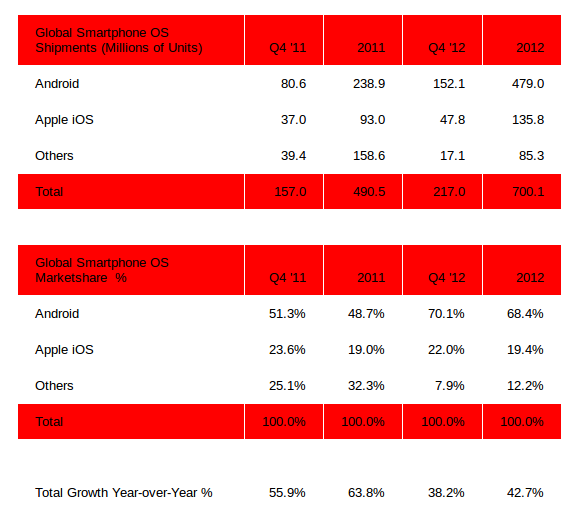
\includegraphics[width=14cm]{img/marche_smartphone.png}
\label{Parts de marché smartphone}
\end{center}

Ces chiffres montrent clairement que le marché des smartphones est très différent du marché du marché des PC, il n’y a pas vraiment de gagnant et les societés voulant profiter ce nouveau canal de communication ont à faire d’importants investissement afin d’être présents dans autant de poches que possible. Beaucoup d’applications doivent être écrite dans au moins deux ou trois plateformes (généralement iOS, Android et Blackberry) pour atteindre une tranche non négligeable du marché.

Actuellement les smartphone ont conquéri le marché des téléphones portables ces dernières années.

Beaucoup de choses ont changé depuis 2007, mais comme comme pour son homologue de bureau, le Web apparaît comme la solution multiplateforme la plus importante à la dispositions des développeurs d’aujourd’hui.

\subsection{La croissance du Web mobiles}

Une des avancées de cette nouvelle génération d’appareils mobiles est la disponibilité d’utiliser pleinement un véritable navigateur Web mobiles, compatible avec la plupart des normes actuelles telles que HTML5, CSS, JavaScript et de nombreux autres standard.

Beaucoup d’entre nous se souviennent regarder Steve Jobs présentant les capacités du navigateur Safari mobile dans le premier iPhone, tout en reconnaissant qu’une nouvelle ère avait commencé précisément ce jour-là.

Les navigateurs mobiles n'étaient pas seulement aussi capable que leurs homologues de bureau, ils étaient meilleurs que les pc , ils étaient rapide et étaient entièrement conformes aux normes.

La montée en puissance de l’internet mobile a apporté de nouvelles possibilités, en particulier dans les pays à faibles pénétration technologique comme l’Amérique latine ou l’Afrique. Les smartphone apparaissent alors comme un bien beaucoup moins cher pour accéder aux informations et services en ligne.

Exemple, en 2010, plus de 30\% de tout les accès web à partir de l’Afrique était fait à partir d’un smartphone.

Dans le monde, on estime que plus de 50\% de tout les requêtes web viendront d’appareils mobile d’ici 2015.

\subsection{Nouveaux paradigmes}

Tout cela représente un énorme changement dans nos habitudes de développer des logiciels.

Un changement radical indiquant  que le web mobile est en train de devenir le nouveau canal principal de la présence du web. L’utilisation de la bande passante à partir d’un pc va être inférieur à celle du mobile.

Mais cette nouvelle perspective pose quelques questions:

\begin{itemize}

  \item
  Combien de plateforme je dois tester pour mon site web?

  \item
  Dois-je me soucier des téléphones mobiles bas de gamme?

  \item
  Quel bibliothèques puis-je utiliser pour accélérer mon développement?

  \item
  Quel est le niveau de support des standard dans les principaux navigateurs mobiles.

\end{itemize}
Pour ce faire, nous allons étudier les technologies suivantes, qui sont actuellement très prometteuses et qui ont une feuille de route très interessantes


\begin{itemize}

  \item[\textbullet]
  PhoneGap

  \item[\textbullet]
  Sencha Touch

  \item[\textbullet]
  Jquery Mobile

\end{itemize}

Il y’a bien sur d’autres technologies intéressantes mais je vais me limiter à l’étude de ces 3 frameworks.



\chapter{Phonegap}
\label{ch:phonegap}

\section*{Introduction}

Développer des applications pour les appareils mobiles peut être fait en utilisant différentes approches et langages. La plupart des applications sont développées en native, ce qui signifie qu’ils sont développés en Java, Objective C, ou un autre langage compris par le SDK disponible dans l’appareil.

Alors que le développement natif permet une plus grande flexibilité et de meilleure performance, le problème se pose lorsque vous souhaitez déplacer une application d’une plate-forme à l’autre. Tout d’un coup vous écrivez l’application presque à partir de zéro. Alors si vous voulez passer à une autre plateforme la même chose se produit.

Il doit y’avoir une meilleure façon de faire !

Toutes les plateformes mobiles actuels supportent l’utilisation d’application web. Ce sont des applications codés entièrement en HTML, JavaScript. Pour des applications simples, ou pour des applications qui n’ont pas besoin d’interagir avec les cappacités de l’appareil, cela fonctionne très bien. Mais au moment où vous avez besoin d’accéder au système de fichiers, travailler avec la caméra, l’accéléromètre ou d’autre composants de l’appareil, vous commencez à avoir un plus grand accès à l’appareil.

C’est la qu’intervient PhoneGap.


\begin{center}
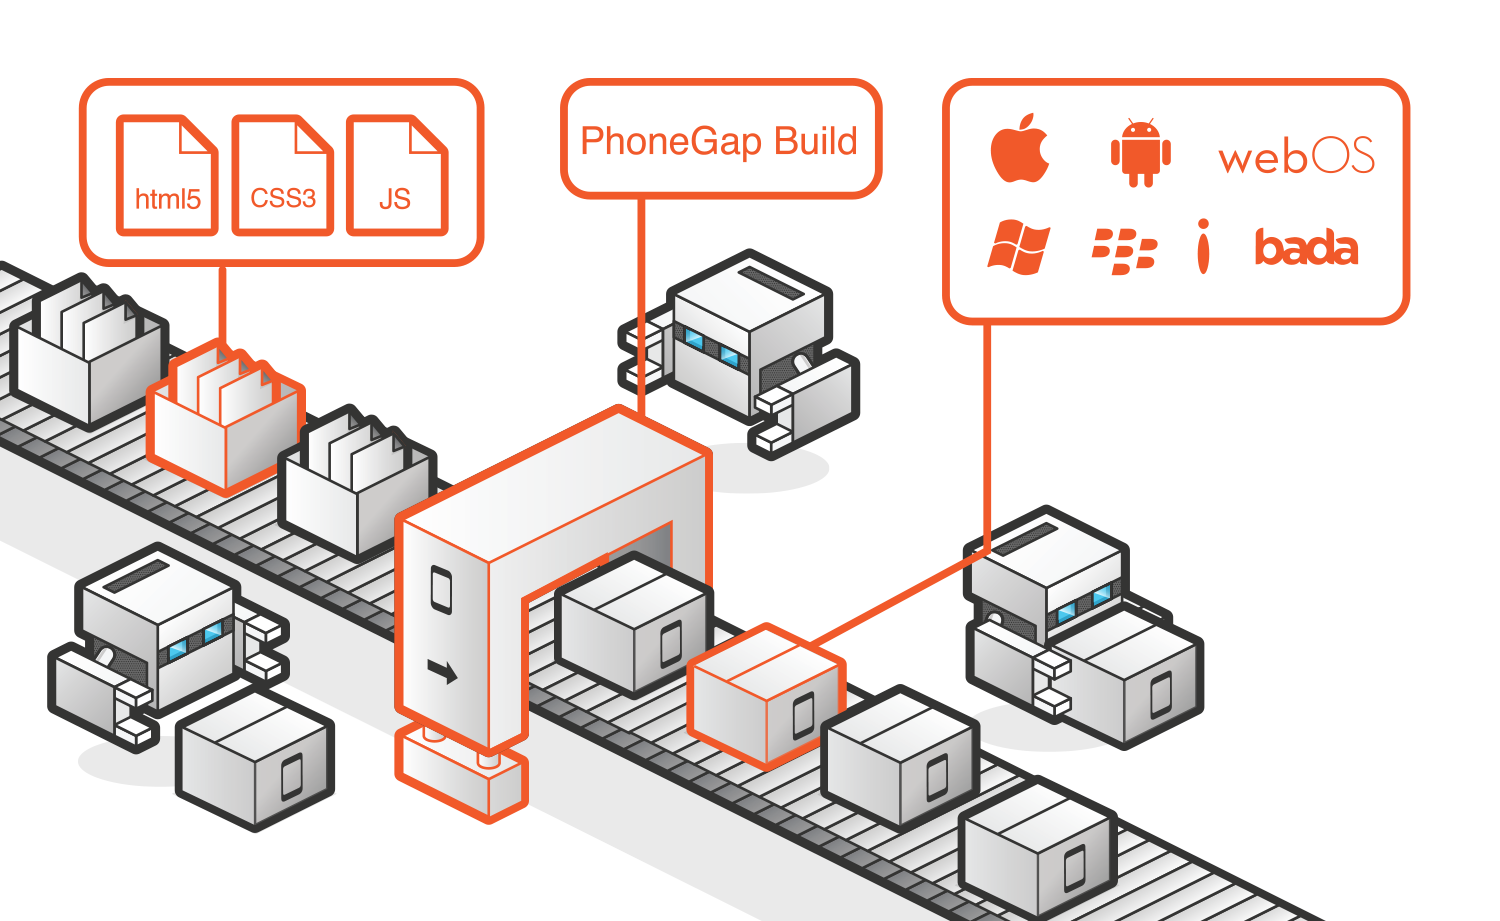
\includegraphics[width=14cm]{img/phonegap.png}
\label{Plateforme Wakanda}
\end{center}


Lorsque vous utilisez l’api de PhoneGap, vous pouvez écrire votre application sans écrire de code natif (Java. Objectif-C, etc). Au lieu de cela, les technologies web sont utilisés, et sont hébérgés en local dans l’application elle même. Et parce que ces API JavaScript sont compatibles sur toutes les plateformes mobiles et construites sur les standards du Web, l’application doit être portable sur les plateformes des appareils avec peu ou pas de modifications.

PhoneGap enveloppe votre HTML et votre JavaScript avec juste assez de code natif pour que votre application web se sente plus à l’aise sur l’appareil. Cette enveloppe est différente pour chaque plateforme, mais elle expose ses capacitées commune de manière cohérente. Cela vous permet de d’écrire moins de code sur de multiples plateformes.

PhoneGap est disponible sur les plateformes suivantes: iOS, Android, Blackberry, Windows Phone, Palm WebOS, Bada et Symbian.

Depuis que PhoneGap enveloppe votre code HTML et JavaScript dans une application native, vous gagnez la possibilité de soumettre votre application au store de l’appareil. Chose que vous ne pouvez pas faire avec une application web simple. Gardez à l’esprit, cependant, que la plupart des store veulent que votre application est le style d’une application native et que certains store sont plus strict que d’autres.

Voici une liste des composants supporté par PhoneGap.

\begin{center}
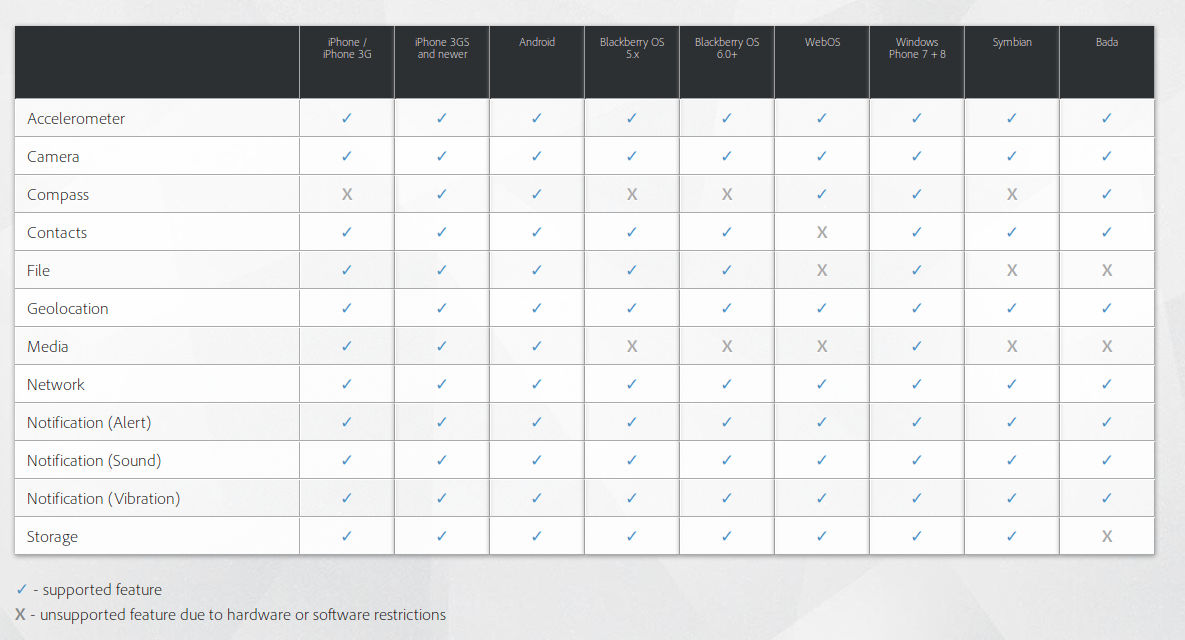
\includegraphics[width=14cm]{img/phonegapFeatures.png}
\label{Plateforme Wakanda}
\end{center}
\section{SenchaTouch}
\label{ch:senchaTouch}

\subsection{Introduction}

Sencha Touch est un framework MVC spécialement conçu pour créer des applications web mobile pour les appareils tactile. Sencha Touch permet aux développeurs de créer des applications pour les plateformes mobiles qui disposent de navigateurs supportant les derniers standards, comme le moteur de rendu Webkit.

Au moment d’écrire ces lignes, la dernière version disponible de Sencha Touch étail la version 2.2.0

Sencha Touch est un gros framework, qui peut sembler intimidant pour les développeurs JavaScript habitués à utiliser des petites bibliothèques telles que jQuery ou Prototype.

Sencha Touch est conçu comme un tout, y compris la plupart des fonctions des services offerts par d’autres frameworks, et il peut être facilement étendu de nombreuses et différentes façon pour s’adapter aux besoins des développeurs de différents domaines d’expertises

Vous n’avez généralement pas besoin d’utiliser d’autres bibliothèques que Sencha Touch dans votre projet, si vous avez besoin d’une fonction particulière vous êtes sûr que le framework l’embarque par défaut.

Le choix explicite de Webkit est intéressante, l’équipe de Sencha Touch a pris une décision délibéré de ne pas soutenir d’autres moteurs de navigateurs mobile, tels que Gecko (Firefox), Presto (Opéra), ou Trident (Internet Explorer). Le soutient exclusif des navigateurs modernes permet à Sencha Touch d’utiliser de nombreuses technologies Web les plus avancées.

Ce choix influe également sur l’expérience du développeur, parce que Safari ou Google Chrome peuvent être utilisé pour déboguer les applications Sencha Touch sur un environnement de bureau comme Linux, Windows ou OS X.

L’équipe de Sencha a récemment annoncé le support d'Internet Explorer 10 pour Windows Phone 8.

Quel type d’application peut-on écrire avec Sencha Touch.

Apple, dans l’une des premières version de son guide sur les directives de design pour IOS a énoncé qu’il existe trois grands types d’applications moblles qui peuvent être créé pour l’iPhone.


\begin{itemize}

  \item[\textbullet]
  les applications utilitaires, comme la météo ou les informations d’informations de stock.

  \item[\textbullet]
  Les applications de productions, comme les applications d’affaires ou orientés document.

  \item[\textbullet]
  Les applications immersives comme les jeux vidéo.

\end{itemize}

Suite à cette taxonomie simple, Sencha Touch est plus apapté pour des applications délivrant les deux premiers types. Bien qu’il est certainement possible de créer des jeux ou d’autres types d’applications mettant en vedette des expériences utilisateurs complexe, ce mémoire ne couvre que la problématique des applications des deux premiers types.

\subsection{Un peu d’histoire}

Retour en 2005, le mouvement web 2.0 est en train de transformer radicalement la notion de contenu web. Les sites en AJAX comme Gmail ont montré au public qu’un nouveau type d’interaction était possible, qu’un nouveau type de contenu a pu être proposé dans les pages web classiques sans l’aide d'extension propriétaires. Douglas Crockford expliquait que JavaScript était un grand langage incompris par beaucoup, et les bibliothèques comme Script.aculo.us et Prototype offrait aux développeurs de concrètes et solides raison pour développer des applications cross-plateformes.

Au milieu de toute cette agitation , Yahoo a publié la première version de sa bibliothèque YUI, permettant de développer des applications complexes à la “desktop-like” à travers les systèmes d’exploitations et navigateurs. YUI peut être considéré comme une œuvre précurseur, après quoi plusieurs autres bibliothèques sont apparus au fil des ans.

Pendant ce temps, Jack Slocum a commencé à travailler sur un ensemble d’extensions pour YUI appelé YUI-Ext. Après quelques versions, l’interêt pour sa bibliothèques a tellement augmenté qu’il à supprimé l’obligation d’utiliser YUI en complément, rendant la bibliothèque en mesure d’utiliser Prototype et/ou YUI pour un niveau de compatiblité cross-plateformes.

\subsection{Ext JS est né}

Pendant des années, Ext JS a établi la norme en terme de compatibilité cross-browser et de conception, permettant aux développeurs de créer des applications de navigation complexe en une fraction de temps, et sans avoir à se soucier des problèmes de compatibilité entre navigateurs. En 2009, la société derrière Ext JS incorporé comme Sencha Inc, dont le siège se trouve à Redwood City, en Californie.

En 2009, la hausse des martphone à écran tactile et, plus tard, ‘liPad, a incité l’équipe d’ Ext JS à créer une version du framework orienté exclusivement pour ces nouveaux dispositifs: le résultat de leurs efforts est Sencha Touch, sortie en version1.0 à la fin 2010.

La première version de Sencha Touch nétait pas totalement compatible avec le version courante d’Ext JS, et il a aussi été critiqué pour ses relatives faibles performance, en particulier sur les anciens appareils tels que l’iPhone 3G. Pour répondre à ces question, Sencha Touch 2 a été publié en Mars 2012 offrant un tout nouveau moteur de rendu basé à 100\% sur Cascading Style Sheet (CSS), et un nouveau système de classe compatible avec Ext JS 4

\subsection{Caractéristiques principales}



Sencha Touch est plus que juste un framework complet orienté vers la création de services et d’applications orienté productivité,  il est en fait un système web complet d’entreprise pour application cross-plateforme, avec 
les caractéristiques suivantes:

\begin{itemize}

  \item[\textbullet]
  Nombreux widget disponibles, largement inspiré par iOS, tant dans la conception que dans les fonctionnalités.

  \item[\textbullet]
  Moteur de rendu rapide basé sur CSS, qui peut être accéléré par le matériel dès les smartphones moderne.

  \item[\textbullet]
  Une architecture bien définie,  Sencha Touch utilise une architecture MVC.

  \item[\textbullet]
  Des connecteurs intégrés pour les serveurs de transfert de données réseau, telles que les services web REST et le soutiens aux application web offline mobile.

  \item[\textbullet]
  Un système de construction de ligne de commande, la gestion de la fusion et de la minification du code de l’application, ainsi que la création d’applications natives pour Android et iOS.

\end{itemize}

Une documentation complète est disponible comme un ensemble de pages HTML dynamiques, y compris la recherche et le filtrage des fonctionnalités sans nécessiter d’infrastructure serveur.

Sencha Touch peut être considéré comme un framework “tout en un”, y compris toutes les API et outils nécessaire pour créer vos applications mobiles.



\subsection{Supprt appareils et navigateurs}

Sencha Touch au moment d’écrire ces lignes ne supporte que les plateformes suivantes:

\begin{itemize}

  \item[\textbullet]
  iOS depuis la version 3

  \item[\textbullet]
  Android depuis la version 2.3

  \item[\textbullet]
  BlackBerry OS depuis la version 6 (uniquement pour les appareils équipés de WebKit)

  \item[\textbullet]
  Windows Phone 8

\end{itemize}

Sencha Touch est un framework basé à 100\% sur le navigateurs, et vous pouvez déployer vos applications Sencha Touch en utilisant n’importe quelle technologie coté serveur, à l’instar de PHP, Java, Ruby on Rails, .Net ou tout autre langage de votre choix.


\subsection{Licence}

Sencha Touch est disponible sous plusieurs licences:

Pour des projets open-source:

\begin{itemize}

  \item[\textbullet]
  Si vous prévoyer de distribuer votre application en divulgant pleinement le code source, il y’a une version de Sencha Touch distribué sous licence GPLv3

  \item[\textbullet]
  Si vous ne souhaitez pas utiliser la licence GPLv3, vous pouvez également utiliser la licence FLOSS.
\end{itemize}



Pour des projets commerciaux:
\begin{itemize}
  \item[\textbullet]
  Vous pouvez utiliser Sencha Touch gratuitement, sans aucun frais que se soit par applications, par utilisateur ou par développeur

  \item[\textbullet]
  Pour les applications embarquées, vous pouvez utiliser Sencha Touch gratuitement jusqu’à 5000 installations.

\end{itemize}
  
Enfin, une licence OEM commercial est disponible aussi bien pour les entreprises désireuses de distribuer Sencha Touch comme une partie de leurs propres applications ou services commerciales.




\section{JQuery Mobile}
\label{ch:jquery mobile}

\subsection{Introduction}

jQuery mobile est un framework open source JavaScript UI construit sur la populaire bibliothèque jQuery, créé par John Resig au cours de la dernière décennie.

Le développement de jQuery mobile a commencé mi-2010, et est rapidement devenu l’un des frameworks JavaScript les plus populaires. Aujourd’hui jQuery Mobile est utilisé dans plus d’application web mobile que n'importe quel autres framework.

jQuery Mobile est un projet open source, hébergé sur Github et avec un site internet très complet, énormément de documentation, d’éxemples et de références à des applications créées avec ce framework.
Au moment d’écrire ces ligne, la version actuelle de jQuery Mobile est la version  1.3.1.

\subsection{Plateformes supportés}

jQuery Mobile fonctionne sur la grande majorité des pc moderne, smartphone et tablette et des plateformes eReader.

En outre, les téléphones et les navigateurs plus ancien sont également supportés en raison d’une évolution progressive. C’est probablement l’une des caractéristiques les plus importes de jQuery Mobile

\subsection{Compatibilité}

Les utilisateurs des navigateurs mobiles les plus avancés peuvent profiter de l’une expérience plus complète, avec des transitions de pages animées basées sur Ajax. Au moment d’écrire ces lignes cette liste comprend les systèmes / navigateurs suivant

\begin{itemize}
  \item[\textbullet]
  iOS depuis la version 3.2
  
  \item[\textbullet]
  Android depuis la version 2.1
  
  \item[\textbullet]
  Windows Phone depuis la version 7
  
  \item[\textbullet]
  BlackBerry depuis la version 6, notament Playbook
  
  \item[\textbullet]
  Palm WebOS depuis la version 1.4
  
  \item[\textbullet]
  Firefox mobile depuis le 10 bêta
  
  \item[\textbullet]
  Skyfire depuis la version 4.1
  
  \item[\textbullet]
  Meego depuis la version 1.2
  
  \item[\textbullet]
  Samsung Bada depuis la version 2.0
  
  \item[\textbullet]
  Navigateur UC 
  
  \item[\textbullet]
  Kindle et Kindle Fire

  \item[\textbullet]
  Nook Color depuis la version 1.4.1

\end{itemize}

Une liste impressionante! Toutes les plateformes importantes de smartphone à écran tactile sont aujourd’hui disponilbe et sont représentée et soutenue par jQuery Mobile.

Sur les plateformes de bureau, jQuery Mobile est compatible avec Windows, Linux et Mac OS X sur les versions des navigateurs suivants:

\begin{itemize}
  \item[\textbullet]
  Firefox depuis la version 4
  
  \item[\textbullet]
  Chrome depuis la version 11
  
  \item[\textbullet]
  Safari deuis la version 4
  
  \item[\textbullet]
  Internet Explorer depuis la version 7
  
  \item[\textbullet]
  Opéra depuis la version 10

\end{itemize}


Un des plus grands avantages en regardant les listes ci-dessus, c’est que jQuery Mobile est l’un des frameworks les plus largement compatibles aujourd’hui. Même mieux, son grand suport des navigateurs de bureau permettent aux développeurs d’utiliser différentes plateformes pour construire et tester leurs applications.

Etant donné que les versions les plus récentes de ces navigateurs intègrent des outils de développement, elle augmentent aussi sont attrait auprès des développeurs.

\subsection{Compatibilités avec les anciennes plateformes mobiles}

Mais que faire si nos utilisateurs ou les exigences précisent certaines anciennes plateforme?

Est-ce que jQuery Mobile peut nous aider dans ce cas?

Les applications jQuery Mobile sont construit avec une dégration progessive par défaut. Les anciennes plateformes, incapable d’afficher les dernières normes CSS et JavaScript, vont tranquillement affichés par défaut la structure HTML des applications, ce qui pourrait ou non être la solution idéale, mais est au moins une réponse par défaut.
Par exemple, les navigateurs suivants ont une expérience améliorée, à l’execption d’Ajax pour la navigation:

\begin{itemize}
  \item[\textbullet]
  BlackBerry 5.0
  
  \item[\textbullet]
  Opera Mini 5.0 à 6.5
  
  \item[\textbullet]
  Nokia Synbian 3
\end{itemize}

Et quelques autres navigateurs ne peuvent profiter que d’une expérience de base en HTML, non amélioré:

\begin{itemize}
  \item[\textbullet]
  BlackBerry 4.x
  
  \item[\textbullet]
  Windows Mobile 6 et plus.
  
  \item[\textbullet]
  Plateformes de smartphone plus anciennes, y compris les téléphones.
  
\end{itemize}

\subsection{Principales caractéristiques}

Une liste succincte des principales caractéristiques de jQuery Mobile

\begin{itemize}
  \item[\textbullet]
  Construit sur la syntaxe de jQuery afin d’avoir une syntaxe familière, cohérente et une courbe d’apprentissage minimale
  
  \item[\textbullet]
  Compatible avec toutes les principales plateformes de bureau et mobiles: iOS, Android, BlackBerry, Palm WebOS, Nokia/Symbian, Windows Mobile, Opera Mobile/Mini, Firefox Mobile, et tout les navigateurs de bureau récent.
  
  \item[\textbullet]
  Léger (environ 20ko une fois compressé avec toutes les fonctionnalités mobile) et minimale
  
  \item[\textbullet]
  Utilisation du HTML5 conduit à un développement des pages rapides et à un minimum de scripting requis.
  
  \item[\textbullet]
  L’utilisation de l’amélioration progressive apporte un contenu de base et de fonctionnalité à tout mobile, tablette ou navigateur avec une expérience riche.
  
  \item[\textbullet]
  Initialisation automatique des widget jQuery en utilisant des attributs HTML dans le code HTML.
  
  \item[\textbullet]
  Des fonctions d'accessibilité telles que WAI-ARIA sont également inclus afin de s’assurer que les pages puissent travailler avec les lecteurs d’écran (par exemple, VoiceOver dans iOS) et d’autres technologies d’assistance.
  
  \item[\textbullet]
  Prise en charge des événements tactile et de la souris en rationalisant le processus du support tactile.
  
\end{itemize}


La chose la plus importante à savoir sur jQuery Mobile est qu’il est une bibliothèque d’interface utilisateur, pas un plugin de jQuery. C’est une bibliothèque qui aura des balises HTML en entrée et utilis des styles prédéfnis en les adaptant aux capacités des navigateurs actuel. Ce n’est pas un framework complet comme .NET, Java, ou encore Sencha Touch qui fournissent des services de niveau inférieur, comme la sérialisation, le stockage ou le réseau.

jQuery mobile s’appuie sur JavaScript et les fonctionnalités du HTML5 prises en charge par le navigateur utilisé.

Cette première caractéristique détermine pourquoi le support des navigateurs mobiles de jQuery Mobile est important comparé aux développeurs Java devant déployer leur propre code pour mettre en œuvre des comportements complexe comme le stockage ou d’intérargir avec le matériel exposés par le navigateur de l’hotes (géolocalisation, boussole, etc)

Une autre caractéristique importante de jQuery Mobile est qu’elle n’impose aucune sorte de structure du code JavaScript dans votre application, la principale composante de l’application étant les fichiers HTML qui défnissent la sémantique de l’interface utilisateur, mais pas son look. En général, les développeurs s’appliqueront à utiliser le comportement de jQuery en utilisant sa norme, sa syntaxe comme avec n’importe qu’elle page web ordinaire.
\section{Conclusion}
\label{ch:conclusion smartphone}




%plateforme
\chapter{Wakanda}
\label{ch:wakanda}

\section*{Introduction}

Wakanda est une plateforme Open Source qui propose une dual licence, avec des capacités de développement strictement identique dans les deux cas. La création ‘une communauté d’utilisateurs et contributeurs est clairement l’ambition première affichée par l’éditeur de Wakanda, dans le but de garantir la pérennité des projets et de s’adapter au foisonnement d’idées, de frameworks, d’appareils et d’usages qui se déroule sous nos yeux.


 
\begin{center}
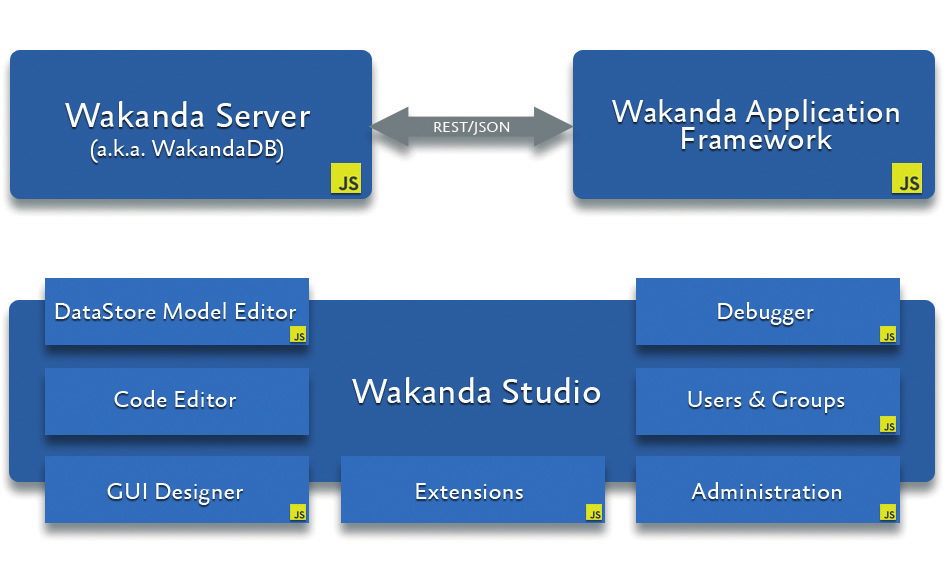
\includegraphics[scale=0.4]{img/wakanda.png}
\label{Plateforme Wakanda}
\end{center}




Au coeur de la plateforme se niche WakandaDBn un datastore objet NoSQL ultra-performant, qui, joint au moteur d’exécution JavaScript, basé sur Webkit, et à un serveur HTTP communiquant via JSON/REST constitue Wakanda Server, le back-end multi-plateformes (Linux, Mac, Windows) qui permettra d’héberger une solution Wakanda sur un serveur dédié, sur un Cloud privé ou public, en mode SaaS, etc...

Le framework Wakanda est automatique déployé vers les clients HTML et embarque un Data Provider qui se comporte comme un proxy des différentes DataClasses générées coté serveur. Ainsi de façon transparente, tous les objets JavaScript générés à l’aide du modèle de données sont expoitables via les différents widgets fournis avec le framework, mais également au travers de requêtes REST pour potentiellement connecter tout type d’interface, par ligne de commande ou à l’aide d’adaptateurs que pourront fournir des tierces parties, la communauté, ou l’éditeur 4D lui-même.
Enfin, le studio Wakanda vient compléter la suite de développement en proposant un IDE dédié capable de contrôler, via une application Desktop Mac ou Windows, aussi bien le modèle, les widgets, et l’adaptation cross-device de chaque écran coté client. Le studio fait la part belle à la gestion graphique du projet, et fait en sorte d’économiser à chaque étape l’écriture de code «technique». Le développeur peut dès lors se concentrer sur ses propres scripts et méthodes qui contiendront l’intelligence métier qui fera la valeur de son application. Outre les différents éditeurs (modèles, code, UI, utilisateurs et groupes) le studio propose une fenêtre d’administration des solutions et projets et un débuggeur qui permet de tracer le code JavaScript tournant sur le serveur. L’installation, tout comme le déploiement, s’effectuent par drag-and- drop d’un package sans aucune configuration. L’hébergement d’une solution Wakanda peut s’effectuer sur un serveur dédié, sur un VPS (serveur dédié virtuel)(2), ou même sur une plateforme IaaS Cloud comme Amazon EC2 ou Rackspace. Côté mobile, Wakanda permet de réaliser des applications Web ou Hybrides, c’est-à-dire embarquées dans un runtime natif généré par PhoneGap. Il est également possible de créer des applications mobiles natives et d’accéder au Serveur via ses API REST et JSON-RPC.


%futur
\chapter{Futur}

\section{Ecmascript6}
\label{ch:ecmascript6}

\subsection{Présentation}


JavaScript a parcouru un long chemin depuis ses humbles débuts il y’a à peu prêt vingt ans. Aujourd’hui , les développeurs sont en train d’écrire des milliers de ligne de code qui créent des applications JavaScript complexes. Avant de nous plonger dans les caractéristiques de ES6, vous pouvez regarder le tableau d’ensemble qui est défini dans le projet de spécifications, en termes d'exigences, d’objectifs , de moyen et de thèmes bordés.

L’un des objectifs de ES6 est d’être un meilleur langage pour la création:


\begin{list}{•}{}
  \item 
  applications complexes
  \item
  bibliothèques
  \item
  générateurs de code
\end{list}

\subsection {Compatibilité}

Le tableau de compatibilité  d’ES6 est très utile, car elle nous indique les caractéristiques pris en charge dans le s navigateurs actuel. Elle nous donne également un lien pratique pour les spécifications de chacun des caractéristiques énumérées.

\begin{center}
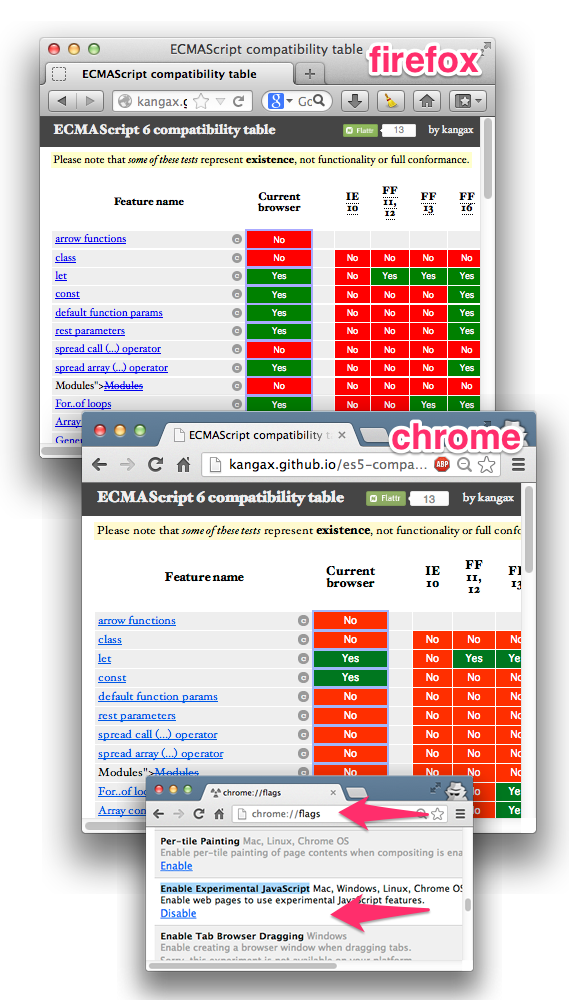
\includegraphics[scale=0.7]{img/es6-compatibility.png}
\label{Plateforme Wakanda}
\end{center}

\subsection{Nouveautés}

Voici ure liste non exhaustive des fonctionnalités qu’apporte EcmaScript 6

\begin{list}{•}{•}
  
  \item 
  Block scoping with let (en utilisant Firefox )
  \item
  Bloc scoping with const (en utilisant Chome )
  \item
  Classes (en utilisant Traceur)
  \item
  Default function parameters (en utilisant TypeScript)
  \item
  Collections (en utilisant NodeJS)
  \item
  Destructuring (en utilisant Firefox)
  \item
  Rest parameters \& Spead operator (en utilisant Grunt plugin Traceur)
  \item
  Iterators (en utilisant Firefox)
  \item
  Array compréhension (en utilisant Firefox)
  \item
  Modules (en utilisant ES6 Module Tranpiler)

\end{list}





%conclusion
\chapter{Conclusion}

À travers ce mémoire, nous avons pu voir que JavaScript a un très fort potentiel dans le développement 3-tiers d'application multi-plateformes. Nous avons abordé les principaux composant de l'architecture 3-tiers et de comment JavaScript peut répondre à chaque composant. Ainsi nous avons pu voir que JavaScript à une réponse pour chaque problématique.

Le JavaScript,a de nombreux atouts, notamment son interopérabilité sur l'ensemble des navigateurs récents du marché et sa bataille importante pour toujours plus de performance et de fonctionnalités mené par Google Chrome et Mozilla Firefox.


JavaScript a actuellement un regain d'actualité avec l'explosion du marché des smartphones et la multiplication des navigateurs mobiles et des systèmes d'exploitation. De plus l'arrivé de nouveaux concurrents comme Tizen, Ubuntu Touch et Firefox OS va stimuler la concurrence autour du développement d'application multi-plateformes.

Le JavaScript avec Node.js s'invite du coté du serveur et répond à une forte demande concernant les applications temps réel et à forte demande. Node.js possède un nombre impressionnant de module et est un des dépôts les plus suivis sur github. La feuille de route de Node.js pour la version 1.0 est impressionnante ce qui reste prometteur pour son avenir.

Les développeurs du libre ont particulièrement bien compris ce nouveau besoin. Si l’on regarde les statistiques de Github, JavaScript représente 21\% des projets hébergés. Ce qui montre la tendance du libre à utilisé massivement JavaScript dans l’avenir.

Les systèmes d'exploitations ont également bien saisi cette tendance en misant également sur le JavaScript pour le développement de leur application. Ainsi Microsoft inclus le support de JavaScript dans Windows 8 et à ainsi introduit le premier langage non développer par la firme.

Néanmoins tout n'est pas forcément au mieux avec la version actuelle de JavaScript et de nombreuse entreprises proposent des alternatives à du JavaScript brut. CoffeeScript (Dropbox) et TypeScript (Microsoft) sont des surcouches de JavaScript afin de permettre au développeurs de coder plus efficacement que ne leur permet JavaScript et ainsi répondre aux principales critiques effectuer sur le code JavaScript. Google propose Dart, un concurrent direct de JavaScript, qui n'a jamais réussi à percer. 

Heureusement EcmaScript Harmony, va permettre à JavaScript d'être plus adapté dans la création d'application en JavaScript et la plupart des navigateurs le supporte déjà. Ainsi avec la nouvelle version Harmony orienté application,la question de ce mémoire sur JavaScript, est il uniquement un langage web ne devrait plus être valable officiellement. Pour l'instant au vu des frameworks disponibles la réponse est non mais ce n'est pas une version officielle.

L'avenir de JavaScript dans les 5 prochaines années sera marqué par l'évolution des moteurs JavaScript et aussi par l'activité autour de Node.js coté serveur ce qui en fait un acteur majeur des prochaines années. Mais est-ce une tendance pour les 5 prochaines année à venir comme l'a été Python ou Ruby ou un sérieux changement pour le développement d'application 3-tiers?
 
\index{blabla}
 
%\listoffigures
%\listoftables
\printindex
\end{document}